% =============================================================================
%  Mathematics Accelerator - Unity Side Report (FIRST DRAFT)
%  EEE2/EIE2 Electronics Design Project
%
%  This file is self-contained and compiles on Overleaf with pdfLaTeX.
%  It follows the AGREED TEAM REPORT STRUCTURE so it can be dropped straight
%  into the shared document. Sections owned by other team members (the
%  mathematical model and the FPGA microarchitecture) are included as short
%  placeholder stubs marked with TODO so the document stays coherent and
%  compiles; the Unity / user-interface content is written in full.
%
%  To merge into the team document: either % =============================================================================
%  Mathematics Accelerator - Unity Side Report (FIRST DRAFT)
%  EEE2/EIE2 Electronics Design Project
%
%  This file is self-contained and compiles on Overleaf with pdfLaTeX.
%  It follows the AGREED TEAM REPORT STRUCTURE so it can be dropped straight
%  into the shared document. Sections owned by other team members (the
%  mathematical model and the FPGA microarchitecture) are included as short
%  placeholder stubs marked with TODO so the document stays coherent and
%  compiles; the Unity / user-interface content is written in full.
%
%  To merge into the team document: either % =============================================================================
%  Mathematics Accelerator - Unity Side Report (FIRST DRAFT)
%  EEE2/EIE2 Electronics Design Project
%
%  This file is self-contained and compiles on Overleaf with pdfLaTeX.
%  It follows the AGREED TEAM REPORT STRUCTURE so it can be dropped straight
%  into the shared document. Sections owned by other team members (the
%  mathematical model and the FPGA microarchitecture) are included as short
%  placeholder stubs marked with TODO so the document stays coherent and
%  compiles; the Unity / user-interface content is written in full.
%
%  To merge into the team document: either % =============================================================================
%  Mathematics Accelerator - Unity Side Report (FIRST DRAFT)
%  EEE2/EIE2 Electronics Design Project
%
%  This file is self-contained and compiles on Overleaf with pdfLaTeX.
%  It follows the AGREED TEAM REPORT STRUCTURE so it can be dropped straight
%  into the shared document. Sections owned by other team members (the
%  mathematical model and the FPGA microarchitecture) are included as short
%  placeholder stubs marked with TODO so the document stays coherent and
%  compiles; the Unity / user-interface content is written in full.
%
%  To merge into the team document: either \input{unity_report} the relevant
%  sections, or copy Sections 2.2, 5.1, 5.2 and 6.4 across.
% =============================================================================

\documentclass[11pt,a4paper]{article}

% ---------- packages -------------------------------------------------------
\usepackage[utf8]{inputenc}
\usepackage[T1]{fontenc}
\usepackage{lmodern}
\usepackage[margin=2.4cm]{geometry}
\usepackage{amsmath,amssymb}
\usepackage{graphicx}
\usepackage{booktabs}
\usepackage{xcolor}
\usepackage{listings}
\usepackage{tikz}
\usetikzlibrary{arrows.meta,positioning,fit,backgrounds}
\usepackage{caption}
\usepackage{siunitx}
\usepackage{enumitem}
\usepackage[hidelinks]{hyperref}

% ---------- code-listing style --------------------------------------------
\definecolor{codebg}{rgb}{0.97,0.97,0.97}
\definecolor{codekw}{rgb}{0.10,0.30,0.65}
\definecolor{codecomment}{rgb}{0.35,0.55,0.35}
\definecolor{codestr}{rgb}{0.70,0.20,0.20}

\lstdefinestyle{code}{
  backgroundcolor=\color{codebg},
  basicstyle=\ttfamily\footnotesize,
  keywordstyle=\color{codekw}\bfseries,
  commentstyle=\color{codecomment}\itshape,
  stringstyle=\color{codestr},
  numbers=left,
  numberstyle=\tiny\color{gray},
  breaklines=true,
  showstringspaces=false,
  frame=single,
  rulecolor=\color{gray!40},
  tabsize=2,
  captionpos=b,
}
\lstset{style=code}

\newcommand{\todo}[1]{\textcolor{red!75!black}{\textbf{[TODO: #1]}}}
\newcommand{\owned}[1]{\textit{\small(Section owned by #1 -- placeholder for integration.)}}

% ---------- title ----------------------------------------------------------
\title{\textbf{Mathematics Accelerator: Real-Time Magnetic-Pendulum Basin Visualiser}\\[4pt]
\large Interactive Visualisation and Control --- Unity User Interface}
\author{\todo{Author name and CID} \\ EEE2/EIE2 Electronics Design Project}
\date{\today}

\begin{document}
\maketitle

% =========================================================================
\begin{abstract}
This project implements an educational \emph{mathematics accelerator} that
visualises, in real time, the basins of attraction of a damped magnetic
pendulum. The function $a=f(x,y)$, where $(x,y)$ is the pendulum's initial
displacement and $a$ encodes the magnet it eventually settles on, is
embarrassingly parallel and computationally intensive, making it an ideal
demonstrator for a custom FPGA datapath on the PYNQ-Z1 platform. This report
focuses on the \textbf{interactive visualisation and control} layer: a Unity
application that renders the accelerator's output as a colour-coded 2D basin
map and a 3D iteration-count height field, lets the user manipulate the
physical parameters of the simulation through sliders, and tracks physical
magnet tokens placed on a board using ArUco-marker computer vision. The Unity
client communicates with the FPGA over a lightweight binary TCP protocol for
image and parameter traffic, and consumes magnet positions produced by the
vision pipeline. We describe the architecture of the front end, the design
decisions that keep the interface responsive (background networking,
parameter throttling, frame versioning), and an end-to-end latency
instrumentation harness. \todo{Add one headline quantitative result, e.g.
median slider-to-image latency in ms once measured.}
\end{abstract}

% =========================================================================
\section{Introduction}

\subsection{Motivation}
The brief asks for an educational tool that visualises a computationally
intensive mathematical function in real time, using an FPGA accelerator to
achieve the throughput required for fluid human interaction. We chose the
\emph{basin of attraction of a magnetic pendulum}: a pendulum bob is released
from rest at an initial position $(x_0,y_0)$ above a set of magnets, and we
colour each starting pixel by which magnet the bob finally settles on. The
result is a fractal-like image whose boundaries are extremely sensitive to
initial conditions, so it is visually striking, genuinely educational
(it illustrates sensitive dependence, damping and attractors), and a stern
test of compute throughput because every pixel requires its own independent
time-marched ODE integration.

A static image, however, is only half of an educational tool. The learning
value comes from \emph{interaction}: seeing how the basin boundaries reorganise
as the damping, magnet strength or pendulum geometry change, and --- most
intuitively --- physically moving the magnets and watching the basins follow.
The Unity user interface exists to make this interaction immediate, legible and
enjoyable, and to present the accelerator's raw output in forms (2D colour map,
3D surface, overlays) that build intuition.

\subsection{System Overview}
\label{sec:system-overview}
The system is composed of three cooperating subsystems connected as shown in
Figure~\ref{fig:dataflow}:

\begin{enumerate}[noitemsep]
  \item \textbf{FPGA accelerator (PYNQ-Z1).} Computes the basin image
        $f(x,y)$ in custom soft logic and exposes it, together with a parameter
        interface, to the rest of the system. \owned{FPGA team}
  \item \textbf{Computer-vision / control software.} An ArUco-marker pipeline
        detects physical magnet tokens on a board, rectifies their positions
        into simulation coordinates, and publishes them. \owned{vision/PYNQ team}
  \item \textbf{Unity user interface.} Renders the basin image, drives the
        physical parameters via sliders, displays tracked magnet positions, and
        offers 2D/3D navigation. This is the subject of this report.
\end{enumerate}

\paragraph{Data flow (as built).}
The Unity client maintains a persistent \textbf{binary TCP} connection to the
board for the two high-rate, latency-critical streams: it \emph{receives} basin
images and \emph{sends} pendulum parameters. Magnet positions originate from the
vision pipeline and are obtained by Unity over a separate lightweight HTTP
endpoint; Unity then relays the same magnet coordinates to the board over the
TCP link so that the FPGA computes the basin for exactly the magnet layout the
user sees on screen. Crucially --- and unlike an earlier iteration of the design
--- \textbf{Flask is no longer used to stream the image or the pendulum
parameters}; those now travel directly over the TCP protocol, and the HTTP
endpoint carries only the ArUco-derived magnet positions.

\begin{figure}[t]
\centering
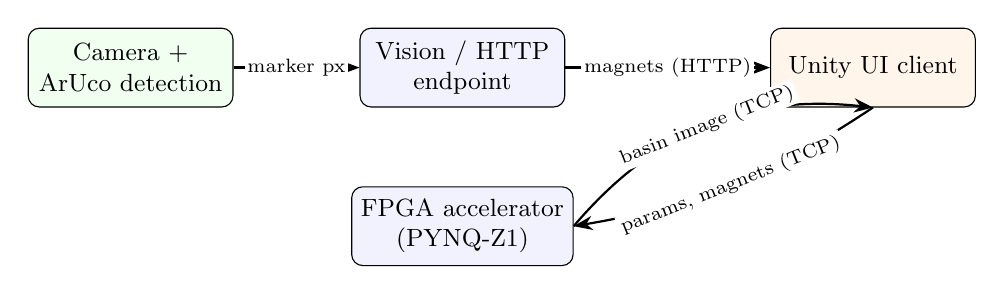
\begin{tikzpicture}[
  node distance=10mm and 16mm,
  box/.style={draw, rounded corners, align=center, minimum height=10mm,
              minimum width=26mm, font=\small, fill=blue!5},
  cam/.style={draw, rounded corners, align=center, minimum height=10mm,
              minimum width=26mm, font=\small, fill=green!6},
  ui/.style={draw, rounded corners, align=center, minimum height=10mm,
              minimum width=26mm, font=\small, fill=orange!8},
  arr/.style={-{Stealth[length=2.4mm]}, thick},
  lbl/.style={font=\scriptsize, fill=white, inner sep=1pt}
]
\node[cam] (cam) {Camera +\\ ArUco detection};
\node[box, right=of cam] (vision) {Vision / HTTP\\ endpoint};
\node[box, below=of vision] (fpga) {FPGA accelerator\\ (PYNQ-Z1)};
\node[ui, right=26mm of vision] (unity) {Unity UI client};

\draw[arr] (cam) -- node[lbl]{marker px} (vision);
\draw[arr] (vision) -- node[lbl, sloped]{magnets (HTTP)} (unity);
\draw[arr] (unity.south) to[bend left=12] node[lbl,sloped]{params, magnets (TCP)} (fpga.east);
\draw[arr] (fpga.east) to[bend left=28] node[lbl,sloped]{basin image (TCP)} (unity.south);
\end{tikzpicture}
\caption{System data flow. High-rate image and parameter traffic uses a binary
TCP protocol between Unity and the FPGA; magnet positions are produced by the
ArUco vision pipeline and consumed (then relayed) by Unity.}
\label{fig:dataflow}
\end{figure}

\subsection{Project Management}
\owned{whole team -- summarise framework, roles and contingencies here}
\todo{Add the role matrix, Gantt/Kanban summary and risk register. The
UI author's role: design and implementation of the Unity front end, the
binary TCP client, parameter-control UX, 2D/3D visualisation and the latency
instrumentation harness; collaboration on the wire protocol and coordinate
conventions shared with the FPGA and vision teams.}

% =========================================================================
\section{Mathematical Model and Reference}
\owned{maths/modelling team}
The Unity interface treats the FPGA output as opaque pixel data, but the
front-end design (colour palettes, height scaling, coordinate mapping and
parameter ranges) is driven by the model below, so it is summarised here for
self-containedness. \todo{Expand each subsection; the parameter values quoted
match the floating-point golden reference in the repository.}

\subsection{Continuous-Time Model}
The bob position $(x,y)$ obeys a damped oscillator with central restoring force
and an attractive force toward each in-plane magnet $i$ at $(a_i,b_i)$:
\begin{align}
\ddot{x} &= -\gamma\dot{x} - \omega^2 x
   - \sum_i \mu\,\frac{x-a_i}{\big((x-a_i)^2+(y-b_i)^2+h^2\big)^{3/2}}, \\
\ddot{y} &= -\gamma\dot{y} - \omega^2 y
   - \sum_i \mu\,\frac{y-b_i}{\big((x-a_i)^2+(y-b_i)^2+h^2\big)^{3/2}},
\end{align}
where $\gamma$ is the damping factor, $\omega^2$ the restoring coefficient,
$\mu$ the magnet strength and $h^2$ the squared bob--magnet plane separation
(kept positive to avoid a singularity). The golden reference uses
$\gamma=0.20$, $\omega^2=1.00$, $h^2=0.25$, $\mu=1.00$, and three magnets on an
equilateral triangle at $(1,0)$ and $(-\tfrac12,\pm\tfrac{\sqrt3}{2})$.

\subsection{Discrete-Time Approximation}
The reference integrates with semi-implicit (symplectic) Euler at step
$\Delta t = 0.01$:
\[
v_{n+1}=v_n+\Delta t\,a(x_n,v_n),\qquad x_{n+1}=x_n+\Delta t\,v_{n+1},
\]
which maps cleanly onto an FPGA datapath of registers, multipliers, adders and
a LUT/approximation for the inverse-power magnet term. \owned{FPGA team for the
hardware mapping}

\subsection{Settle and Timeout Conditions}
A pixel is classified once the bob stays within $r_\text{settle}=0.10$ of a
magnet \emph{and} below $v_\text{settle}=0.01$ in speed for
$3$ consecutive steps, or on timeout at $\text{max\_steps}=5000$. The iteration
count at settling is exported alongside the basin label and is what the Unity
3D view renders as height.

\subsection{Floating-Point Reference Model}
\owned{maths team} A NumPy float64 model is the functional golden reference;
\todo{cross-reference figure of the reference basin image.}

\subsection{Parameter Selection}
The render window is the square $[-1.8,1.8]^2$ in simulation units; this exact
constant ($1.8$) is reused throughout the Unity coordinate mappings and the
ArUco homography target so that pixel, simulation and board coordinates agree.
\todo{Justify word-length / bit-depth selection here (links to Section 4).}

% =========================================================================
\section{Accelerator Microarchitecture}
\owned{FPGA team -- full content}
\todo{This section is authored by the FPGA team. The only interface that the
Unity client depends on is summarised in Section~\ref{sec:protocol}: a binary
image frame (width, height, bit depth, version, packed pixels) and a parameter
register update. Keep the pixel encoding (Section~\ref{sec:pixeldecode}) in sync
with the hardware.}

\subsection{Pixel Scanner and Coordinate Mapper}\owned{FPGA team}
\subsection{Fixed-Point Number Representation}\owned{FPGA team}
\subsection{LUT-Based Force Approximation}\owned{FPGA team}
\subsection{Pipelined Pendulum Solver}\owned{FPGA team}
\subsection{Parallel Solver Architecture}\owned{FPGA team}
\subsection{AXI-Lite Control Interface}\owned{FPGA team}
\subsection{VDMA Data Transfer}\owned{FPGA team}

% =========================================================================
\section{Interactive Visualisation \& Control}

\subsection{Python/PYNQ Control Software}
\owned{PYNQ/vision team -- written here from the UI's perspective}
From the Unity client's perspective the control software provides two services.
First, a TCP server on the board accepts the binary protocol of
Section~\ref{sec:protocol}, forwards parameter and magnet updates to the
accelerator, and streams completed basin frames back. Second, the ArUco vision
pipeline (Section~\ref{sec:magnets}) detects physical magnet tokens, rectifies
their image coordinates onto the simulation plane via a homography, and exposes
them on a lightweight HTTP endpoint that Unity polls. \todo{PYNQ team to detail
the server, threading and overlay binding. The websocket hub
(\texttt{ws/\{client\}}) is the intended convergence point for ArUco, Unity and
FPGA clients and should be described if it is part of the final build.}

% -------------------------------------------------------------------------
\subsection{Unity-Based User Interface}
\label{sec:unity}

The user interface is a Unity application (Universal Render Pipeline) whose
responsibilities are: (i) maintain a robust connection to the FPGA;
(ii) present the basin image in two complementary visual forms; (iii) let the
user manipulate the model parameters with immediate visual feedback;
(iv) integrate physical magnet tracking; and (v) provide 2D/3D navigation.
The code is deliberately modular --- one ``concern'' per
\texttt{MonoBehaviour} --- so that the networking, control, rendering and
camera logic can be developed and tested independently. Table~\ref{tab:scripts}
lists the components.

\begin{table}[h]
\centering
\caption{Unity components and responsibilities.}
\label{tab:scripts}
\small
\begin{tabular}{@{}lp{10.4cm}@{}}
\toprule
\textbf{Script} & \textbf{Responsibility} \\
\midrule
\texttt{PynqConnection} & Background-threaded binary TCP client; frame
codec; auto-reconnect; outbound parameter/magnet sending; main-thread event
marshalling. \\
\texttt{PynqParamController} & Throttles and de-duplicates slider-driven
parameter updates before they are sent. \\
\texttt{SliderTextDisplay} & Maps a normalised UI slider to a physical
parameter range, formats the readout, raises change/release events. \\
\texttt{PendulumRenderer} & Decodes each pixel into (basin, iteration count);
builds the 2D category and value textures and the 3D height-field mesh. \\
\texttt{MagnetRenderer} & Polls the vision endpoint for magnet positions,
draws them on a mini-map, and relays them to the FPGA. \\
\texttt{PanZoom} & Pan/zoom of the 2D simulation window, constrained to the
valid simulation bounds. \\
\texttt{OrbitCamera} & Orbit/pan/zoom camera for the 3D surface view. \\
\texttt{ViewManager} & Switches between the 2D and 3D presentations. \\
\texttt{ImagePostToFrameTimer}, \texttt{SliderToImageTimer} & Latency
instrumentation (local render time and end-to-end round trip). \\
\texttt{VertexColor} (shader) & Minimal URP shader that renders the 3D mesh
using per-vertex basin colours. \\
\bottomrule
\end{tabular}
\end{table}

% --------------------------------------------------
\subsubsection{Networking layer and wire protocol}
\label{sec:protocol}

All latency-critical traffic uses a single persistent TCP connection
(\texttt{PynqConnection}). A custom binary framing was chosen over JSON-over-HTTP
because a basin frame is dense numeric data sent many times per second; framing
it as raw bytes avoids both per-frame connection overhead and the
serialisation cost of text formats. Every frame is:
\[
\underbrace{\texttt{type}}_{1\,\text{byte}}\;
\underbrace{\texttt{length}}_{4\,\text{bytes, big-endian}}\;
\underbrace{\texttt{payload}}_{\texttt{length bytes}}
\]
with message types \texttt{PARAMS} (\texttt{0x01}) and \texttt{MAGNETS}
(\texttt{0x02}) outbound, and \texttt{IMAGE} (\texttt{0x10}) and \texttt{INFO}
(\texttt{0x11}) inbound. An image payload begins with a 9-byte header
(\texttt{u16} width, \texttt{u16} height, \texttt{u8} bit depth, \texttt{u32}
version) followed by packed pixels (one byte each at $\le 8$ bits, otherwise
two bytes big-endian). Parameter and magnet payloads are compact JSON.

\paragraph{Threading.}
Networking runs on a dedicated background thread so that a blocking socket read
never stalls Unity's render loop. Decoded messages are pushed onto a
lock-free \texttt{ConcurrentQueue} and drained in \texttt{Update()}, guaranteeing
that all \texttt{ImageReceived}/\texttt{InfoReceived} events fire on the Unity
main thread where it is safe to touch \texttt{Texture2D} and \texttt{Mesh}
objects (Listing~\ref{lst:io}). The connection self-heals: on any socket error
the loop closes the stream, waits a configurable interval, and reconnects,
flushing any pending parameter frame on reconnection.

\begin{lstlisting}[language=Java,caption={Background receive loop drained on the main thread (\texttt{PynqConnection}).},label={lst:io}]
// background thread: read framed messages, enqueue for main thread
private void ReadFrames() {
    byte[] header = new byte[5];
    while (running) {
        ReadExactly(header, 5);
        byte type = header[0];
        int length = (int)ReadU32BE(header, 1);
        byte[] payload = length > 0 ? new byte[length] : Array.Empty<byte>();
        if (length > 0) ReadExactly(payload, length);
        if (type == MSG_IMAGE) inbound.Enqueue(DecodeImage(payload));
        else if (type == MSG_INFO) inbound.Enqueue(DecodeInfo(payload));
    }
}
// main thread (Update): raise events where Unity objects are safe to touch
while (inbound.TryDequeue(out object msg)) { /* invoke ImageReceived / InfoReceived */ }
\end{lstlisting}

\paragraph{Frame versioning.}
Each parameter update carries an incrementing \texttt{version}, and the client
records the minimum image version it is willing to accept afterwards. Incoming
frames older than this watermark are discarded in \texttt{PendulumRenderer}, so
the display never briefly shows a stale basin produced before the latest slider
change took effect --- important when the user drags a slider and several
in-flight frames are still arriving.

% --------------------------------------------------
\subsubsection{Parameter control and UX}
\label{sec:params}

Four parameters --- damping factor, magnet strength, pendulum length and
pendulum height --- are exposed as sliders. \texttt{SliderTextDisplay} maps the
slider's normalised $[0,1]$ value onto the parameter's physical
$[\text{min},\text{max}]$ range, rounds to two decimals for a stable readout,
and raises two signals: a \emph{changed} signal on every move and a
\emph{released} signal on pointer-up.

A na\"ive design would transmit a parameter frame on every slider callback,
flooding the link and the accelerator while the user drags. Instead,
\texttt{PynqParamController} \textbf{throttles} sends to at most one every
\SI{0.1}{s} while dragging, and on release forces an immediate final send so the
last value is never lost. It also \textbf{de-duplicates}: if a snapshot equals
the last value actually sent (or a value already queued), it is dropped. This
gives responsive dragging without saturating the FPGA, and guarantees the steady
state always reflects the slider exactly. The combination of throttle +
forced-flush-on-release is a deliberate latency/throughput trade-off and is
discussed in Section~\ref{sec:tradeoffs}.

% --------------------------------------------------
\subsubsection{Basin visualisation: 2D textures and 3D surface}
\label{sec:pixeldecode}

\texttt{PendulumRenderer} subscribes to \texttt{ImageReceived} and, for each
frame, converts the packed pixels into three views. Every pixel encodes two
quantities: the \emph{basin label} (which magnet won) and the \emph{iteration
count} (how long the bob took to settle, i.e.\ how close to a boundary the
starting point was). The decode is bit-depth aware so the same front end works
with the current 6-bit hardware output and a future 14-bit mode:

\begin{lstlisting}[language=Java,caption={Bit-depth-aware pixel decode (\texttt{PendulumRenderer}).},label={lst:decode}]
static void DecodePixel(int pixel, int bitDepth, out int category, out int depth) {
    if (bitDepth <= 6) { category = pixel & 0x3;          depth = (pixel >> 2) & 0xF; }
    else               { category = (pixel >> 12) & 0x3;  depth = pixel & 0xFFF; }
}
\end{lstlisting}

\paragraph{2D category map.}
The basin label indexes a small palette (one colour per magnet, dark grey for
unresolved), producing the familiar tri-colour basin image. Array rows are
flipped vertically to match Unity's bottom-left texture origin.

\paragraph{2D value map.}
The iteration count is normalised to $[0,255]$ and passed through a
\emph{plasma} colour map (a perceptually-ordered gradient interpolated between
nine anchor colours). This exposes the fractal boundary structure --- regions
that take many iterations to settle glow brightly --- which the flat category
map hides.

\paragraph{3D height field.}
The same per-pixel data builds a triangulated mesh: $(x,y)$ are the pixel
coordinates and the height is the iteration count, scaled per bit depth. Vertices
are coloured by basin label and drawn with the minimal \texttt{VertexColor} URP
shader, giving an interactive 3D ``landscape'' whose peaks are the
sensitive basin boundaries. A \texttt{UInt32} index buffer is used so the mesh
can exceed 65k vertices at full resolution, and the mesh skeleton (triangle
indices) is rebuilt only when the frame dimensions change, not every frame.

% --------------------------------------------------
\subsubsection{Physical magnet tracking integration}
\label{sec:magnets}

\texttt{MagnetRenderer} closes the loop between the physical board and the
simulation. It polls the vision endpoint (default every \SI{0.5}{s}) for the
current magnet dictionary, maps each magnet's simulation coordinate
($[-1.8,1.8]$) onto a $130\times130$ mini-map and draws it as a coloured disc,
then relays the same coordinates to the FPGA over TCP
(\texttt{SendMagnets}). The vision side derives these coordinates from ArUco
markers: four corner markers (IDs 0--3) define a homography that rectifies the
camera image to the square board, and three token markers (IDs 4--6) are the
movable magnets, whose centres are transformed into simulation units before
publishing. Because Unity both \emph{displays} and \emph{forwards} the magnet
positions, the on-screen dots and the FPGA's computed basin are always
consistent.

% --------------------------------------------------
\subsubsection{Navigation and view management}

Two camera/navigation behaviours serve the two views. \texttt{PanZoom} (2D)
implements scroll-to-zoom and drag-to-pan over the simulation window using
Unity's Input System, clamping the requested window so it can never leave the
valid simulation bounds $[-1.8,1.8]^2$ (a minimum half-size prevents zooming in
past the point where the image becomes blocky). \texttt{OrbitCamera} (3D)
provides orbit (left-drag), pan (right-drag) and zoom (scroll) around the height
field. \texttt{ViewManager} toggles between the 2D canvas and the 3D overlay,
enabling the orbit camera only in 3D. \todo{Confirm whether the pan/zoom window
is forwarded to the FPGA to re-render at higher resolution, or is a local
view-only crop; describe accordingly.}

% --------------------------------------------------
\subsubsection{Design decisions and trade-offs}
\label{sec:tradeoffs}

\begin{itemize}[noitemsep]
  \item \textbf{Binary TCP vs.\ HTTP/JSON for frames.} Dense, high-rate pixel
        data is sent as packed bytes over one persistent socket, eliminating
        per-frame connection setup and text-parsing overhead. Low-rate,
        human-readable data (parameters, magnets) stays as small JSON payloads
        inside the same framing for convenience.
  \item \textbf{Background I/O + main-thread marshalling.} Keeps the render loop
        free of blocking socket calls while respecting Unity's rule that scene
        objects are touched only on the main thread.
  \item \textbf{Throttle + de-duplicate + flush-on-release.} Bounds the
        parameter update rate during dragging (protecting the link and the
        accelerator) while guaranteeing the final value always lands.
  \item \textbf{Frame versioning watermark.} Prevents stale frames from
        flashing on screen after a parameter change, at the cost of occasionally
        discarding a just-too-old frame.
  \item \textbf{Bit-depth-aware decode.} One renderer supports both the present
        6-bit and a future 14-bit hardware output without code changes,
        decoupling UI development from the FPGA's numeric format.
  \item \textbf{Two visual encodings + 3D.} The category map answers ``which
        magnet?'', the plasma value map and 3D surface answer ``how chaotic
        here?'', directly serving the educational objective.
\end{itemize}

% =========================================================================
\section{Verification and Evaluation}

\subsection{Evaluation Strategy Linked to Design Objectives}
The UI's objectives --- responsiveness, faithful presentation of the
accelerator output, robust connectivity and intuitive control --- map onto
measurable tests: end-to-end latency (slider-to-image), local render time,
reconnection behaviour, and correctness of the pixel decode against the golden
reference. \todo{Tabulate each requirement against its test and pass criterion.}

\subsection{Software Model Validation}
\owned{maths team} Validation of the floating-point reference and the
fixed-point model against it. \todo{cross-reference.}

\subsection{Submodule Testing}
The Python services that the UI depends on are unit-tested (the Flask state
model, magnet add/remove/update, parameters and \texttt{/info} construction have
a \texttt{pytest} suite). On the Unity side, the pixel decode and coordinate
mappings are deterministic pure functions and were checked against the golden
reference's encoding; the networking codec was exercised against
\todo{describe: loopback test / recorded frames}. \todo{Add ArUco accuracy test
(reprojection error of known marker layout).}

\subsection{System Performance Evaluation}
Two lightweight stopwatches instrument the live system without external tools.
\texttt{SliderToImageTimer} starts when a slider changes and stops when an image
with a newer version is rendered, giving the \textbf{end-to-end round-trip
latency} (UI $\rightarrow$ FPGA $\rightarrow$ UI). \texttt{ImagePostToFrameTimer}
measures the \textbf{local processing time} from a TCP frame arriving to the
textures and mesh being updated, isolating the UI's own contribution from the
network/compute path. Together they decompose total latency into ``UI render''
and ``everything else''. \todo{Insert the measured distributions (median,
p95) for 6-bit $160\times120$ frames; compare 2D-only vs.\ 2D+3D rendering
cost; state the achieved interactive frame rate.}

% =========================================================================
\section*{References}
\todo{Add bibliography (PYNQ docs, ArUco/OpenCV, Unity URP, plasma colormap
source). Consider switching to \texttt{biblatex} when integrating with the team
document.}

% =========================================================================
\appendix
\section{Wire Protocol Summary}
\begin{table}[h]
\centering
\small
\begin{tabular}{@{}llp{7.6cm}@{}}
\toprule
\textbf{Type} & \textbf{Dir} & \textbf{Payload} \\
\midrule
\texttt{0x01 PARAMS}  & UI$\to$FPGA & JSON: version, dampingFactor,
magneticStrength, pendulumLength, pendulumHeight \\
\texttt{0x02 MAGNETS} & UI$\to$FPGA & JSON: \{ magnets: \{ magnet\_i: \{x,y\} \} \} \\
\texttt{0x10 IMAGE}   & FPGA$\to$UI & 9-byte header (w,h,depth,version) +
packed pixels \\
\texttt{0x11 INFO}    & FPGA$\to$UI & JSON: magnet dictionary \\
\bottomrule
\end{tabular}
\caption{Binary framing: 1-byte type, 4-byte big-endian length, payload.}
\end{table}

\section{Key Source Files}
\todo{Optionally include trimmed listings of \texttt{PynqConnection.cs},
\texttt{PendulumRenderer.cs} and \texttt{PynqParamController.cs}, or reference
the repository.}

\end{document}
 the relevant
%  sections, or copy Sections 2.2, 5.1, 5.2 and 6.4 across.
% =============================================================================

\documentclass[11pt,a4paper]{article}

% ---------- packages -------------------------------------------------------
\usepackage[utf8]{inputenc}
\usepackage[T1]{fontenc}
\usepackage{lmodern}
\usepackage[margin=2.4cm]{geometry}
\usepackage{amsmath,amssymb}
\usepackage{graphicx}
\usepackage{booktabs}
\usepackage{xcolor}
\usepackage{listings}
\usepackage{tikz}
\usetikzlibrary{arrows.meta,positioning,fit,backgrounds}
\usepackage{caption}
\usepackage{siunitx}
\usepackage{enumitem}
\usepackage[hidelinks]{hyperref}

% ---------- code-listing style --------------------------------------------
\definecolor{codebg}{rgb}{0.97,0.97,0.97}
\definecolor{codekw}{rgb}{0.10,0.30,0.65}
\definecolor{codecomment}{rgb}{0.35,0.55,0.35}
\definecolor{codestr}{rgb}{0.70,0.20,0.20}

\lstdefinestyle{code}{
  backgroundcolor=\color{codebg},
  basicstyle=\ttfamily\footnotesize,
  keywordstyle=\color{codekw}\bfseries,
  commentstyle=\color{codecomment}\itshape,
  stringstyle=\color{codestr},
  numbers=left,
  numberstyle=\tiny\color{gray},
  breaklines=true,
  showstringspaces=false,
  frame=single,
  rulecolor=\color{gray!40},
  tabsize=2,
  captionpos=b,
}
\lstset{style=code}

\newcommand{\todo}[1]{\textcolor{red!75!black}{\textbf{[TODO: #1]}}}
\newcommand{\owned}[1]{\textit{\small(Section owned by #1 -- placeholder for integration.)}}

% ---------- title ----------------------------------------------------------
\title{\textbf{Mathematics Accelerator: Real-Time Magnetic-Pendulum Basin Visualiser}\\[4pt]
\large Interactive Visualisation and Control --- Unity User Interface}
\author{\todo{Author name and CID} \\ EEE2/EIE2 Electronics Design Project}
\date{\today}

\begin{document}
\maketitle

% =========================================================================
\begin{abstract}
This project implements an educational \emph{mathematics accelerator} that
visualises, in real time, the basins of attraction of a damped magnetic
pendulum. The function $a=f(x,y)$, where $(x,y)$ is the pendulum's initial
displacement and $a$ encodes the magnet it eventually settles on, is
embarrassingly parallel and computationally intensive, making it an ideal
demonstrator for a custom FPGA datapath on the PYNQ-Z1 platform. This report
focuses on the \textbf{interactive visualisation and control} layer: a Unity
application that renders the accelerator's output as a colour-coded 2D basin
map and a 3D iteration-count height field, lets the user manipulate the
physical parameters of the simulation through sliders, and tracks physical
magnet tokens placed on a board using ArUco-marker computer vision. The Unity
client communicates with the FPGA over a lightweight binary TCP protocol for
image and parameter traffic, and consumes magnet positions produced by the
vision pipeline. We describe the architecture of the front end, the design
decisions that keep the interface responsive (background networking,
parameter throttling, frame versioning), and an end-to-end latency
instrumentation harness. \todo{Add one headline quantitative result, e.g.
median slider-to-image latency in ms once measured.}
\end{abstract}

% =========================================================================
\section{Introduction}

\subsection{Motivation}
The brief asks for an educational tool that visualises a computationally
intensive mathematical function in real time, using an FPGA accelerator to
achieve the throughput required for fluid human interaction. We chose the
\emph{basin of attraction of a magnetic pendulum}: a pendulum bob is released
from rest at an initial position $(x_0,y_0)$ above a set of magnets, and we
colour each starting pixel by which magnet the bob finally settles on. The
result is a fractal-like image whose boundaries are extremely sensitive to
initial conditions, so it is visually striking, genuinely educational
(it illustrates sensitive dependence, damping and attractors), and a stern
test of compute throughput because every pixel requires its own independent
time-marched ODE integration.

A static image, however, is only half of an educational tool. The learning
value comes from \emph{interaction}: seeing how the basin boundaries reorganise
as the damping, magnet strength or pendulum geometry change, and --- most
intuitively --- physically moving the magnets and watching the basins follow.
The Unity user interface exists to make this interaction immediate, legible and
enjoyable, and to present the accelerator's raw output in forms (2D colour map,
3D surface, overlays) that build intuition.

\subsection{System Overview}
\label{sec:system-overview}
The system is composed of three cooperating subsystems connected as shown in
Figure~\ref{fig:dataflow}:

\begin{enumerate}[noitemsep]
  \item \textbf{FPGA accelerator (PYNQ-Z1).} Computes the basin image
        $f(x,y)$ in custom soft logic and exposes it, together with a parameter
        interface, to the rest of the system. \owned{FPGA team}
  \item \textbf{Computer-vision / control software.} An ArUco-marker pipeline
        detects physical magnet tokens on a board, rectifies their positions
        into simulation coordinates, and publishes them. \owned{vision/PYNQ team}
  \item \textbf{Unity user interface.} Renders the basin image, drives the
        physical parameters via sliders, displays tracked magnet positions, and
        offers 2D/3D navigation. This is the subject of this report.
\end{enumerate}

\paragraph{Data flow (as built).}
The Unity client maintains a persistent \textbf{binary TCP} connection to the
board for the two high-rate, latency-critical streams: it \emph{receives} basin
images and \emph{sends} pendulum parameters. Magnet positions originate from the
vision pipeline and are obtained by Unity over a separate lightweight HTTP
endpoint; Unity then relays the same magnet coordinates to the board over the
TCP link so that the FPGA computes the basin for exactly the magnet layout the
user sees on screen. Crucially --- and unlike an earlier iteration of the design
--- \textbf{Flask is no longer used to stream the image or the pendulum
parameters}; those now travel directly over the TCP protocol, and the HTTP
endpoint carries only the ArUco-derived magnet positions.

\begin{figure}[t]
\centering
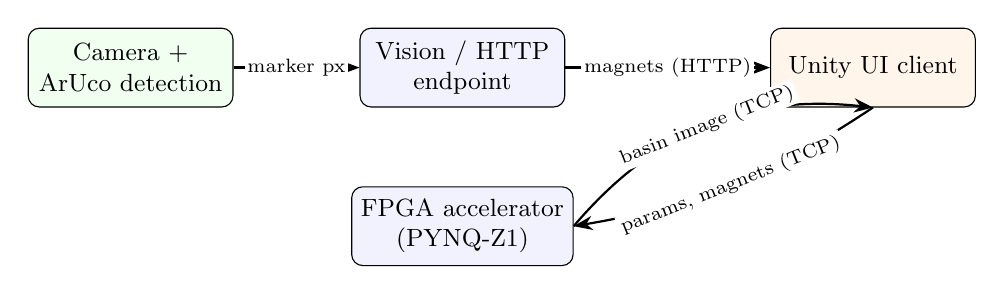
\begin{tikzpicture}[
  node distance=10mm and 16mm,
  box/.style={draw, rounded corners, align=center, minimum height=10mm,
              minimum width=26mm, font=\small, fill=blue!5},
  cam/.style={draw, rounded corners, align=center, minimum height=10mm,
              minimum width=26mm, font=\small, fill=green!6},
  ui/.style={draw, rounded corners, align=center, minimum height=10mm,
              minimum width=26mm, font=\small, fill=orange!8},
  arr/.style={-{Stealth[length=2.4mm]}, thick},
  lbl/.style={font=\scriptsize, fill=white, inner sep=1pt}
]
\node[cam] (cam) {Camera +\\ ArUco detection};
\node[box, right=of cam] (vision) {Vision / HTTP\\ endpoint};
\node[box, below=of vision] (fpga) {FPGA accelerator\\ (PYNQ-Z1)};
\node[ui, right=26mm of vision] (unity) {Unity UI client};

\draw[arr] (cam) -- node[lbl]{marker px} (vision);
\draw[arr] (vision) -- node[lbl, sloped]{magnets (HTTP)} (unity);
\draw[arr] (unity.south) to[bend left=12] node[lbl,sloped]{params, magnets (TCP)} (fpga.east);
\draw[arr] (fpga.east) to[bend left=28] node[lbl,sloped]{basin image (TCP)} (unity.south);
\end{tikzpicture}
\caption{System data flow. High-rate image and parameter traffic uses a binary
TCP protocol between Unity and the FPGA; magnet positions are produced by the
ArUco vision pipeline and consumed (then relayed) by Unity.}
\label{fig:dataflow}
\end{figure}

\subsection{Project Management}
\owned{whole team -- summarise framework, roles and contingencies here}
\todo{Add the role matrix, Gantt/Kanban summary and risk register. The
UI author's role: design and implementation of the Unity front end, the
binary TCP client, parameter-control UX, 2D/3D visualisation and the latency
instrumentation harness; collaboration on the wire protocol and coordinate
conventions shared with the FPGA and vision teams.}

% =========================================================================
\section{Mathematical Model and Reference}
\owned{maths/modelling team}
The Unity interface treats the FPGA output as opaque pixel data, but the
front-end design (colour palettes, height scaling, coordinate mapping and
parameter ranges) is driven by the model below, so it is summarised here for
self-containedness. \todo{Expand each subsection; the parameter values quoted
match the floating-point golden reference in the repository.}

\subsection{Continuous-Time Model}
The bob position $(x,y)$ obeys a damped oscillator with central restoring force
and an attractive force toward each in-plane magnet $i$ at $(a_i,b_i)$:
\begin{align}
\ddot{x} &= -\gamma\dot{x} - \omega^2 x
   - \sum_i \mu\,\frac{x-a_i}{\big((x-a_i)^2+(y-b_i)^2+h^2\big)^{3/2}}, \\
\ddot{y} &= -\gamma\dot{y} - \omega^2 y
   - \sum_i \mu\,\frac{y-b_i}{\big((x-a_i)^2+(y-b_i)^2+h^2\big)^{3/2}},
\end{align}
where $\gamma$ is the damping factor, $\omega^2$ the restoring coefficient,
$\mu$ the magnet strength and $h^2$ the squared bob--magnet plane separation
(kept positive to avoid a singularity). The golden reference uses
$\gamma=0.20$, $\omega^2=1.00$, $h^2=0.25$, $\mu=1.00$, and three magnets on an
equilateral triangle at $(1,0)$ and $(-\tfrac12,\pm\tfrac{\sqrt3}{2})$.

\subsection{Discrete-Time Approximation}
The reference integrates with semi-implicit (symplectic) Euler at step
$\Delta t = 0.01$:
\[
v_{n+1}=v_n+\Delta t\,a(x_n,v_n),\qquad x_{n+1}=x_n+\Delta t\,v_{n+1},
\]
which maps cleanly onto an FPGA datapath of registers, multipliers, adders and
a LUT/approximation for the inverse-power magnet term. \owned{FPGA team for the
hardware mapping}

\subsection{Settle and Timeout Conditions}
A pixel is classified once the bob stays within $r_\text{settle}=0.10$ of a
magnet \emph{and} below $v_\text{settle}=0.01$ in speed for
$3$ consecutive steps, or on timeout at $\text{max\_steps}=5000$. The iteration
count at settling is exported alongside the basin label and is what the Unity
3D view renders as height.

\subsection{Floating-Point Reference Model}
\owned{maths team} A NumPy float64 model is the functional golden reference;
\todo{cross-reference figure of the reference basin image.}

\subsection{Parameter Selection}
The render window is the square $[-1.8,1.8]^2$ in simulation units; this exact
constant ($1.8$) is reused throughout the Unity coordinate mappings and the
ArUco homography target so that pixel, simulation and board coordinates agree.
\todo{Justify word-length / bit-depth selection here (links to Section 4).}

% =========================================================================
\section{Accelerator Microarchitecture}
\owned{FPGA team -- full content}
\todo{This section is authored by the FPGA team. The only interface that the
Unity client depends on is summarised in Section~\ref{sec:protocol}: a binary
image frame (width, height, bit depth, version, packed pixels) and a parameter
register update. Keep the pixel encoding (Section~\ref{sec:pixeldecode}) in sync
with the hardware.}

\subsection{Pixel Scanner and Coordinate Mapper}\owned{FPGA team}
\subsection{Fixed-Point Number Representation}\owned{FPGA team}
\subsection{LUT-Based Force Approximation}\owned{FPGA team}
\subsection{Pipelined Pendulum Solver}\owned{FPGA team}
\subsection{Parallel Solver Architecture}\owned{FPGA team}
\subsection{AXI-Lite Control Interface}\owned{FPGA team}
\subsection{VDMA Data Transfer}\owned{FPGA team}

% =========================================================================
\section{Interactive Visualisation \& Control}

\subsection{Python/PYNQ Control Software}
\owned{PYNQ/vision team -- written here from the UI's perspective}
From the Unity client's perspective the control software provides two services.
First, a TCP server on the board accepts the binary protocol of
Section~\ref{sec:protocol}, forwards parameter and magnet updates to the
accelerator, and streams completed basin frames back. Second, the ArUco vision
pipeline (Section~\ref{sec:magnets}) detects physical magnet tokens, rectifies
their image coordinates onto the simulation plane via a homography, and exposes
them on a lightweight HTTP endpoint that Unity polls. \todo{PYNQ team to detail
the server, threading and overlay binding. The websocket hub
(\texttt{ws/\{client\}}) is the intended convergence point for ArUco, Unity and
FPGA clients and should be described if it is part of the final build.}

% -------------------------------------------------------------------------
\subsection{Unity-Based User Interface}
\label{sec:unity}

The user interface is a Unity application (Universal Render Pipeline) whose
responsibilities are: (i) maintain a robust connection to the FPGA;
(ii) present the basin image in two complementary visual forms; (iii) let the
user manipulate the model parameters with immediate visual feedback;
(iv) integrate physical magnet tracking; and (v) provide 2D/3D navigation.
The code is deliberately modular --- one ``concern'' per
\texttt{MonoBehaviour} --- so that the networking, control, rendering and
camera logic can be developed and tested independently. Table~\ref{tab:scripts}
lists the components.

\begin{table}[h]
\centering
\caption{Unity components and responsibilities.}
\label{tab:scripts}
\small
\begin{tabular}{@{}lp{10.4cm}@{}}
\toprule
\textbf{Script} & \textbf{Responsibility} \\
\midrule
\texttt{PynqConnection} & Background-threaded binary TCP client; frame
codec; auto-reconnect; outbound parameter/magnet sending; main-thread event
marshalling. \\
\texttt{PynqParamController} & Throttles and de-duplicates slider-driven
parameter updates before they are sent. \\
\texttt{SliderTextDisplay} & Maps a normalised UI slider to a physical
parameter range, formats the readout, raises change/release events. \\
\texttt{PendulumRenderer} & Decodes each pixel into (basin, iteration count);
builds the 2D category and value textures and the 3D height-field mesh. \\
\texttt{MagnetRenderer} & Polls the vision endpoint for magnet positions,
draws them on a mini-map, and relays them to the FPGA. \\
\texttt{PanZoom} & Pan/zoom of the 2D simulation window, constrained to the
valid simulation bounds. \\
\texttt{OrbitCamera} & Orbit/pan/zoom camera for the 3D surface view. \\
\texttt{ViewManager} & Switches between the 2D and 3D presentations. \\
\texttt{ImagePostToFrameTimer}, \texttt{SliderToImageTimer} & Latency
instrumentation (local render time and end-to-end round trip). \\
\texttt{VertexColor} (shader) & Minimal URP shader that renders the 3D mesh
using per-vertex basin colours. \\
\bottomrule
\end{tabular}
\end{table}

% --------------------------------------------------
\subsubsection{Networking layer and wire protocol}
\label{sec:protocol}

All latency-critical traffic uses a single persistent TCP connection
(\texttt{PynqConnection}). A custom binary framing was chosen over JSON-over-HTTP
because a basin frame is dense numeric data sent many times per second; framing
it as raw bytes avoids both per-frame connection overhead and the
serialisation cost of text formats. Every frame is:
\[
\underbrace{\texttt{type}}_{1\,\text{byte}}\;
\underbrace{\texttt{length}}_{4\,\text{bytes, big-endian}}\;
\underbrace{\texttt{payload}}_{\texttt{length bytes}}
\]
with message types \texttt{PARAMS} (\texttt{0x01}) and \texttt{MAGNETS}
(\texttt{0x02}) outbound, and \texttt{IMAGE} (\texttt{0x10}) and \texttt{INFO}
(\texttt{0x11}) inbound. An image payload begins with a 9-byte header
(\texttt{u16} width, \texttt{u16} height, \texttt{u8} bit depth, \texttt{u32}
version) followed by packed pixels (one byte each at $\le 8$ bits, otherwise
two bytes big-endian). Parameter and magnet payloads are compact JSON.

\paragraph{Threading.}
Networking runs on a dedicated background thread so that a blocking socket read
never stalls Unity's render loop. Decoded messages are pushed onto a
lock-free \texttt{ConcurrentQueue} and drained in \texttt{Update()}, guaranteeing
that all \texttt{ImageReceived}/\texttt{InfoReceived} events fire on the Unity
main thread where it is safe to touch \texttt{Texture2D} and \texttt{Mesh}
objects (Listing~\ref{lst:io}). The connection self-heals: on any socket error
the loop closes the stream, waits a configurable interval, and reconnects,
flushing any pending parameter frame on reconnection.

\begin{lstlisting}[language=Java,caption={Background receive loop drained on the main thread (\texttt{PynqConnection}).},label={lst:io}]
// background thread: read framed messages, enqueue for main thread
private void ReadFrames() {
    byte[] header = new byte[5];
    while (running) {
        ReadExactly(header, 5);
        byte type = header[0];
        int length = (int)ReadU32BE(header, 1);
        byte[] payload = length > 0 ? new byte[length] : Array.Empty<byte>();
        if (length > 0) ReadExactly(payload, length);
        if (type == MSG_IMAGE) inbound.Enqueue(DecodeImage(payload));
        else if (type == MSG_INFO) inbound.Enqueue(DecodeInfo(payload));
    }
}
// main thread (Update): raise events where Unity objects are safe to touch
while (inbound.TryDequeue(out object msg)) { /* invoke ImageReceived / InfoReceived */ }
\end{lstlisting}

\paragraph{Frame versioning.}
Each parameter update carries an incrementing \texttt{version}, and the client
records the minimum image version it is willing to accept afterwards. Incoming
frames older than this watermark are discarded in \texttt{PendulumRenderer}, so
the display never briefly shows a stale basin produced before the latest slider
change took effect --- important when the user drags a slider and several
in-flight frames are still arriving.

% --------------------------------------------------
\subsubsection{Parameter control and UX}
\label{sec:params}

Four parameters --- damping factor, magnet strength, pendulum length and
pendulum height --- are exposed as sliders. \texttt{SliderTextDisplay} maps the
slider's normalised $[0,1]$ value onto the parameter's physical
$[\text{min},\text{max}]$ range, rounds to two decimals for a stable readout,
and raises two signals: a \emph{changed} signal on every move and a
\emph{released} signal on pointer-up.

A na\"ive design would transmit a parameter frame on every slider callback,
flooding the link and the accelerator while the user drags. Instead,
\texttt{PynqParamController} \textbf{throttles} sends to at most one every
\SI{0.1}{s} while dragging, and on release forces an immediate final send so the
last value is never lost. It also \textbf{de-duplicates}: if a snapshot equals
the last value actually sent (or a value already queued), it is dropped. This
gives responsive dragging without saturating the FPGA, and guarantees the steady
state always reflects the slider exactly. The combination of throttle +
forced-flush-on-release is a deliberate latency/throughput trade-off and is
discussed in Section~\ref{sec:tradeoffs}.

% --------------------------------------------------
\subsubsection{Basin visualisation: 2D textures and 3D surface}
\label{sec:pixeldecode}

\texttt{PendulumRenderer} subscribes to \texttt{ImageReceived} and, for each
frame, converts the packed pixels into three views. Every pixel encodes two
quantities: the \emph{basin label} (which magnet won) and the \emph{iteration
count} (how long the bob took to settle, i.e.\ how close to a boundary the
starting point was). The decode is bit-depth aware so the same front end works
with the current 6-bit hardware output and a future 14-bit mode:

\begin{lstlisting}[language=Java,caption={Bit-depth-aware pixel decode (\texttt{PendulumRenderer}).},label={lst:decode}]
static void DecodePixel(int pixel, int bitDepth, out int category, out int depth) {
    if (bitDepth <= 6) { category = pixel & 0x3;          depth = (pixel >> 2) & 0xF; }
    else               { category = (pixel >> 12) & 0x3;  depth = pixel & 0xFFF; }
}
\end{lstlisting}

\paragraph{2D category map.}
The basin label indexes a small palette (one colour per magnet, dark grey for
unresolved), producing the familiar tri-colour basin image. Array rows are
flipped vertically to match Unity's bottom-left texture origin.

\paragraph{2D value map.}
The iteration count is normalised to $[0,255]$ and passed through a
\emph{plasma} colour map (a perceptually-ordered gradient interpolated between
nine anchor colours). This exposes the fractal boundary structure --- regions
that take many iterations to settle glow brightly --- which the flat category
map hides.

\paragraph{3D height field.}
The same per-pixel data builds a triangulated mesh: $(x,y)$ are the pixel
coordinates and the height is the iteration count, scaled per bit depth. Vertices
are coloured by basin label and drawn with the minimal \texttt{VertexColor} URP
shader, giving an interactive 3D ``landscape'' whose peaks are the
sensitive basin boundaries. A \texttt{UInt32} index buffer is used so the mesh
can exceed 65k vertices at full resolution, and the mesh skeleton (triangle
indices) is rebuilt only when the frame dimensions change, not every frame.

% --------------------------------------------------
\subsubsection{Physical magnet tracking integration}
\label{sec:magnets}

\texttt{MagnetRenderer} closes the loop between the physical board and the
simulation. It polls the vision endpoint (default every \SI{0.5}{s}) for the
current magnet dictionary, maps each magnet's simulation coordinate
($[-1.8,1.8]$) onto a $130\times130$ mini-map and draws it as a coloured disc,
then relays the same coordinates to the FPGA over TCP
(\texttt{SendMagnets}). The vision side derives these coordinates from ArUco
markers: four corner markers (IDs 0--3) define a homography that rectifies the
camera image to the square board, and three token markers (IDs 4--6) are the
movable magnets, whose centres are transformed into simulation units before
publishing. Because Unity both \emph{displays} and \emph{forwards} the magnet
positions, the on-screen dots and the FPGA's computed basin are always
consistent.

% --------------------------------------------------
\subsubsection{Navigation and view management}

Two camera/navigation behaviours serve the two views. \texttt{PanZoom} (2D)
implements scroll-to-zoom and drag-to-pan over the simulation window using
Unity's Input System, clamping the requested window so it can never leave the
valid simulation bounds $[-1.8,1.8]^2$ (a minimum half-size prevents zooming in
past the point where the image becomes blocky). \texttt{OrbitCamera} (3D)
provides orbit (left-drag), pan (right-drag) and zoom (scroll) around the height
field. \texttt{ViewManager} toggles between the 2D canvas and the 3D overlay,
enabling the orbit camera only in 3D. \todo{Confirm whether the pan/zoom window
is forwarded to the FPGA to re-render at higher resolution, or is a local
view-only crop; describe accordingly.}

% --------------------------------------------------
\subsubsection{Design decisions and trade-offs}
\label{sec:tradeoffs}

\begin{itemize}[noitemsep]
  \item \textbf{Binary TCP vs.\ HTTP/JSON for frames.} Dense, high-rate pixel
        data is sent as packed bytes over one persistent socket, eliminating
        per-frame connection setup and text-parsing overhead. Low-rate,
        human-readable data (parameters, magnets) stays as small JSON payloads
        inside the same framing for convenience.
  \item \textbf{Background I/O + main-thread marshalling.} Keeps the render loop
        free of blocking socket calls while respecting Unity's rule that scene
        objects are touched only on the main thread.
  \item \textbf{Throttle + de-duplicate + flush-on-release.} Bounds the
        parameter update rate during dragging (protecting the link and the
        accelerator) while guaranteeing the final value always lands.
  \item \textbf{Frame versioning watermark.} Prevents stale frames from
        flashing on screen after a parameter change, at the cost of occasionally
        discarding a just-too-old frame.
  \item \textbf{Bit-depth-aware decode.} One renderer supports both the present
        6-bit and a future 14-bit hardware output without code changes,
        decoupling UI development from the FPGA's numeric format.
  \item \textbf{Two visual encodings + 3D.} The category map answers ``which
        magnet?'', the plasma value map and 3D surface answer ``how chaotic
        here?'', directly serving the educational objective.
\end{itemize}

% =========================================================================
\section{Verification and Evaluation}

\subsection{Evaluation Strategy Linked to Design Objectives}
The UI's objectives --- responsiveness, faithful presentation of the
accelerator output, robust connectivity and intuitive control --- map onto
measurable tests: end-to-end latency (slider-to-image), local render time,
reconnection behaviour, and correctness of the pixel decode against the golden
reference. \todo{Tabulate each requirement against its test and pass criterion.}

\subsection{Software Model Validation}
\owned{maths team} Validation of the floating-point reference and the
fixed-point model against it. \todo{cross-reference.}

\subsection{Submodule Testing}
The Python services that the UI depends on are unit-tested (the Flask state
model, magnet add/remove/update, parameters and \texttt{/info} construction have
a \texttt{pytest} suite). On the Unity side, the pixel decode and coordinate
mappings are deterministic pure functions and were checked against the golden
reference's encoding; the networking codec was exercised against
\todo{describe: loopback test / recorded frames}. \todo{Add ArUco accuracy test
(reprojection error of known marker layout).}

\subsection{System Performance Evaluation}
Two lightweight stopwatches instrument the live system without external tools.
\texttt{SliderToImageTimer} starts when a slider changes and stops when an image
with a newer version is rendered, giving the \textbf{end-to-end round-trip
latency} (UI $\rightarrow$ FPGA $\rightarrow$ UI). \texttt{ImagePostToFrameTimer}
measures the \textbf{local processing time} from a TCP frame arriving to the
textures and mesh being updated, isolating the UI's own contribution from the
network/compute path. Together they decompose total latency into ``UI render''
and ``everything else''. \todo{Insert the measured distributions (median,
p95) for 6-bit $160\times120$ frames; compare 2D-only vs.\ 2D+3D rendering
cost; state the achieved interactive frame rate.}

% =========================================================================
\section*{References}
\todo{Add bibliography (PYNQ docs, ArUco/OpenCV, Unity URP, plasma colormap
source). Consider switching to \texttt{biblatex} when integrating with the team
document.}

% =========================================================================
\appendix
\section{Wire Protocol Summary}
\begin{table}[h]
\centering
\small
\begin{tabular}{@{}llp{7.6cm}@{}}
\toprule
\textbf{Type} & \textbf{Dir} & \textbf{Payload} \\
\midrule
\texttt{0x01 PARAMS}  & UI$\to$FPGA & JSON: version, dampingFactor,
magneticStrength, pendulumLength, pendulumHeight \\
\texttt{0x02 MAGNETS} & UI$\to$FPGA & JSON: \{ magnets: \{ magnet\_i: \{x,y\} \} \} \\
\texttt{0x10 IMAGE}   & FPGA$\to$UI & 9-byte header (w,h,depth,version) +
packed pixels \\
\texttt{0x11 INFO}    & FPGA$\to$UI & JSON: magnet dictionary \\
\bottomrule
\end{tabular}
\caption{Binary framing: 1-byte type, 4-byte big-endian length, payload.}
\end{table}

\section{Key Source Files}
\todo{Optionally include trimmed listings of \texttt{PynqConnection.cs},
\texttt{PendulumRenderer.cs} and \texttt{PynqParamController.cs}, or reference
the repository.}

\end{document}
 the relevant
%  sections, or copy Sections 2.2, 5.1, 5.2 and 6.4 across.
% =============================================================================

\documentclass[11pt,a4paper]{article}

% ---------- packages -------------------------------------------------------
\usepackage[utf8]{inputenc}
\usepackage[T1]{fontenc}
\usepackage{lmodern}
\usepackage[margin=2.4cm]{geometry}
\usepackage{amsmath,amssymb}
\usepackage{graphicx}
\usepackage{booktabs}
\usepackage{xcolor}
\usepackage{listings}
\usepackage{tikz}
\usetikzlibrary{arrows.meta,positioning,fit,backgrounds}
\usepackage{caption}
\usepackage{siunitx}
\usepackage{enumitem}
\usepackage[hidelinks]{hyperref}

% ---------- code-listing style --------------------------------------------
\definecolor{codebg}{rgb}{0.97,0.97,0.97}
\definecolor{codekw}{rgb}{0.10,0.30,0.65}
\definecolor{codecomment}{rgb}{0.35,0.55,0.35}
\definecolor{codestr}{rgb}{0.70,0.20,0.20}

\lstdefinestyle{code}{
  backgroundcolor=\color{codebg},
  basicstyle=\ttfamily\footnotesize,
  keywordstyle=\color{codekw}\bfseries,
  commentstyle=\color{codecomment}\itshape,
  stringstyle=\color{codestr},
  numbers=left,
  numberstyle=\tiny\color{gray},
  breaklines=true,
  showstringspaces=false,
  frame=single,
  rulecolor=\color{gray!40},
  tabsize=2,
  captionpos=b,
}
\lstset{style=code}

\newcommand{\todo}[1]{\textcolor{red!75!black}{\textbf{[TODO: #1]}}}
\newcommand{\owned}[1]{\textit{\small(Section owned by #1 -- placeholder for integration.)}}

% ---------- title ----------------------------------------------------------
\title{\textbf{Mathematics Accelerator: Real-Time Magnetic-Pendulum Basin Visualiser}\\[4pt]
\large Interactive Visualisation and Control --- Unity User Interface}
\author{\todo{Author name and CID} \\ EEE2/EIE2 Electronics Design Project}
\date{\today}

\begin{document}
\maketitle

% =========================================================================
\begin{abstract}
This project implements an educational \emph{mathematics accelerator} that
visualises, in real time, the basins of attraction of a damped magnetic
pendulum. The function $a=f(x,y)$, where $(x,y)$ is the pendulum's initial
displacement and $a$ encodes the magnet it eventually settles on, is
embarrassingly parallel and computationally intensive, making it an ideal
demonstrator for a custom FPGA datapath on the PYNQ-Z1 platform. This report
focuses on the \textbf{interactive visualisation and control} layer: a Unity
application that renders the accelerator's output as a colour-coded 2D basin
map and a 3D iteration-count height field, lets the user manipulate the
physical parameters of the simulation through sliders, and tracks physical
magnet tokens placed on a board using ArUco-marker computer vision. The Unity
client communicates with the FPGA over a lightweight binary TCP protocol for
image and parameter traffic, and consumes magnet positions produced by the
vision pipeline. We describe the architecture of the front end, the design
decisions that keep the interface responsive (background networking,
parameter throttling, frame versioning), and an end-to-end latency
instrumentation harness. \todo{Add one headline quantitative result, e.g.
median slider-to-image latency in ms once measured.}
\end{abstract}

% =========================================================================
\section{Introduction}

\subsection{Motivation}
The brief asks for an educational tool that visualises a computationally
intensive mathematical function in real time, using an FPGA accelerator to
achieve the throughput required for fluid human interaction. We chose the
\emph{basin of attraction of a magnetic pendulum}: a pendulum bob is released
from rest at an initial position $(x_0,y_0)$ above a set of magnets, and we
colour each starting pixel by which magnet the bob finally settles on. The
result is a fractal-like image whose boundaries are extremely sensitive to
initial conditions, so it is visually striking, genuinely educational
(it illustrates sensitive dependence, damping and attractors), and a stern
test of compute throughput because every pixel requires its own independent
time-marched ODE integration.

A static image, however, is only half of an educational tool. The learning
value comes from \emph{interaction}: seeing how the basin boundaries reorganise
as the damping, magnet strength or pendulum geometry change, and --- most
intuitively --- physically moving the magnets and watching the basins follow.
The Unity user interface exists to make this interaction immediate, legible and
enjoyable, and to present the accelerator's raw output in forms (2D colour map,
3D surface, overlays) that build intuition.

\subsection{System Overview}
\label{sec:system-overview}
The system is composed of three cooperating subsystems connected as shown in
Figure~\ref{fig:dataflow}:

\begin{enumerate}[noitemsep]
  \item \textbf{FPGA accelerator (PYNQ-Z1).} Computes the basin image
        $f(x,y)$ in custom soft logic and exposes it, together with a parameter
        interface, to the rest of the system. \owned{FPGA team}
  \item \textbf{Computer-vision / control software.} An ArUco-marker pipeline
        detects physical magnet tokens on a board, rectifies their positions
        into simulation coordinates, and publishes them. \owned{vision/PYNQ team}
  \item \textbf{Unity user interface.} Renders the basin image, drives the
        physical parameters via sliders, displays tracked magnet positions, and
        offers 2D/3D navigation. This is the subject of this report.
\end{enumerate}

\paragraph{Data flow (as built).}
The Unity client maintains a persistent \textbf{binary TCP} connection to the
board for the two high-rate, latency-critical streams: it \emph{receives} basin
images and \emph{sends} pendulum parameters. Magnet positions originate from the
vision pipeline and are obtained by Unity over a separate lightweight HTTP
endpoint; Unity then relays the same magnet coordinates to the board over the
TCP link so that the FPGA computes the basin for exactly the magnet layout the
user sees on screen. Crucially --- and unlike an earlier iteration of the design
--- \textbf{Flask is no longer used to stream the image or the pendulum
parameters}; those now travel directly over the TCP protocol, and the HTTP
endpoint carries only the ArUco-derived magnet positions.

\begin{figure}[t]
\centering
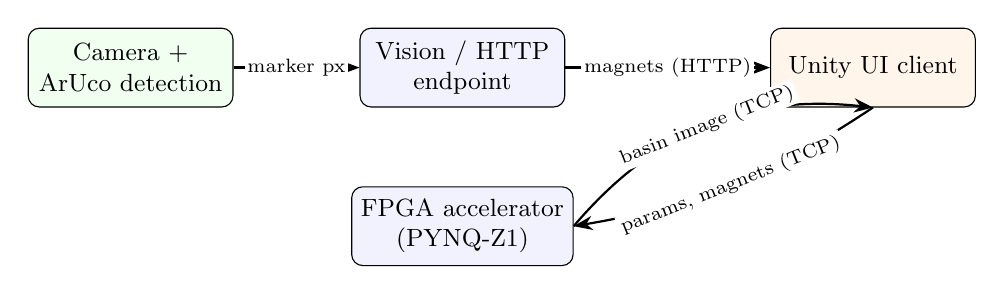
\begin{tikzpicture}[
  node distance=10mm and 16mm,
  box/.style={draw, rounded corners, align=center, minimum height=10mm,
              minimum width=26mm, font=\small, fill=blue!5},
  cam/.style={draw, rounded corners, align=center, minimum height=10mm,
              minimum width=26mm, font=\small, fill=green!6},
  ui/.style={draw, rounded corners, align=center, minimum height=10mm,
              minimum width=26mm, font=\small, fill=orange!8},
  arr/.style={-{Stealth[length=2.4mm]}, thick},
  lbl/.style={font=\scriptsize, fill=white, inner sep=1pt}
]
\node[cam] (cam) {Camera +\\ ArUco detection};
\node[box, right=of cam] (vision) {Vision / HTTP\\ endpoint};
\node[box, below=of vision] (fpga) {FPGA accelerator\\ (PYNQ-Z1)};
\node[ui, right=26mm of vision] (unity) {Unity UI client};

\draw[arr] (cam) -- node[lbl]{marker px} (vision);
\draw[arr] (vision) -- node[lbl, sloped]{magnets (HTTP)} (unity);
\draw[arr] (unity.south) to[bend left=12] node[lbl,sloped]{params, magnets (TCP)} (fpga.east);
\draw[arr] (fpga.east) to[bend left=28] node[lbl,sloped]{basin image (TCP)} (unity.south);
\end{tikzpicture}
\caption{System data flow. High-rate image and parameter traffic uses a binary
TCP protocol between Unity and the FPGA; magnet positions are produced by the
ArUco vision pipeline and consumed (then relayed) by Unity.}
\label{fig:dataflow}
\end{figure}

\subsection{Project Management}
\owned{whole team -- summarise framework, roles and contingencies here}
\todo{Add the role matrix, Gantt/Kanban summary and risk register. The
UI author's role: design and implementation of the Unity front end, the
binary TCP client, parameter-control UX, 2D/3D visualisation and the latency
instrumentation harness; collaboration on the wire protocol and coordinate
conventions shared with the FPGA and vision teams.}

% =========================================================================
\section{Mathematical Model and Reference}
\owned{maths/modelling team}
The Unity interface treats the FPGA output as opaque pixel data, but the
front-end design (colour palettes, height scaling, coordinate mapping and
parameter ranges) is driven by the model below, so it is summarised here for
self-containedness. \todo{Expand each subsection; the parameter values quoted
match the floating-point golden reference in the repository.}

\subsection{Continuous-Time Model}
The bob position $(x,y)$ obeys a damped oscillator with central restoring force
and an attractive force toward each in-plane magnet $i$ at $(a_i,b_i)$:
\begin{align}
\ddot{x} &= -\gamma\dot{x} - \omega^2 x
   - \sum_i \mu\,\frac{x-a_i}{\big((x-a_i)^2+(y-b_i)^2+h^2\big)^{3/2}}, \\
\ddot{y} &= -\gamma\dot{y} - \omega^2 y
   - \sum_i \mu\,\frac{y-b_i}{\big((x-a_i)^2+(y-b_i)^2+h^2\big)^{3/2}},
\end{align}
where $\gamma$ is the damping factor, $\omega^2$ the restoring coefficient,
$\mu$ the magnet strength and $h^2$ the squared bob--magnet plane separation
(kept positive to avoid a singularity). The golden reference uses
$\gamma=0.20$, $\omega^2=1.00$, $h^2=0.25$, $\mu=1.00$, and three magnets on an
equilateral triangle at $(1,0)$ and $(-\tfrac12,\pm\tfrac{\sqrt3}{2})$.

\subsection{Discrete-Time Approximation}
The reference integrates with semi-implicit (symplectic) Euler at step
$\Delta t = 0.01$:
\[
v_{n+1}=v_n+\Delta t\,a(x_n,v_n),\qquad x_{n+1}=x_n+\Delta t\,v_{n+1},
\]
which maps cleanly onto an FPGA datapath of registers, multipliers, adders and
a LUT/approximation for the inverse-power magnet term. \owned{FPGA team for the
hardware mapping}

\subsection{Settle and Timeout Conditions}
A pixel is classified once the bob stays within $r_\text{settle}=0.10$ of a
magnet \emph{and} below $v_\text{settle}=0.01$ in speed for
$3$ consecutive steps, or on timeout at $\text{max\_steps}=5000$. The iteration
count at settling is exported alongside the basin label and is what the Unity
3D view renders as height.

\subsection{Floating-Point Reference Model}
\owned{maths team} A NumPy float64 model is the functional golden reference;
\todo{cross-reference figure of the reference basin image.}

\subsection{Parameter Selection}
The render window is the square $[-1.8,1.8]^2$ in simulation units; this exact
constant ($1.8$) is reused throughout the Unity coordinate mappings and the
ArUco homography target so that pixel, simulation and board coordinates agree.
\todo{Justify word-length / bit-depth selection here (links to Section 4).}

% =========================================================================
\section{Accelerator Microarchitecture}
\owned{FPGA team -- full content}
\todo{This section is authored by the FPGA team. The only interface that the
Unity client depends on is summarised in Section~\ref{sec:protocol}: a binary
image frame (width, height, bit depth, version, packed pixels) and a parameter
register update. Keep the pixel encoding (Section~\ref{sec:pixeldecode}) in sync
with the hardware.}

\subsection{Pixel Scanner and Coordinate Mapper}\owned{FPGA team}
\subsection{Fixed-Point Number Representation}\owned{FPGA team}
\subsection{LUT-Based Force Approximation}\owned{FPGA team}
\subsection{Pipelined Pendulum Solver}\owned{FPGA team}
\subsection{Parallel Solver Architecture}\owned{FPGA team}
\subsection{AXI-Lite Control Interface}\owned{FPGA team}
\subsection{VDMA Data Transfer}\owned{FPGA team}

% =========================================================================
\section{Interactive Visualisation \& Control}

\subsection{Python/PYNQ Control Software}
\owned{PYNQ/vision team -- written here from the UI's perspective}
From the Unity client's perspective the control software provides two services.
First, a TCP server on the board accepts the binary protocol of
Section~\ref{sec:protocol}, forwards parameter and magnet updates to the
accelerator, and streams completed basin frames back. Second, the ArUco vision
pipeline (Section~\ref{sec:magnets}) detects physical magnet tokens, rectifies
their image coordinates onto the simulation plane via a homography, and exposes
them on a lightweight HTTP endpoint that Unity polls. \todo{PYNQ team to detail
the server, threading and overlay binding. The websocket hub
(\texttt{ws/\{client\}}) is the intended convergence point for ArUco, Unity and
FPGA clients and should be described if it is part of the final build.}

% -------------------------------------------------------------------------
\subsection{Unity-Based User Interface}
\label{sec:unity}

The user interface is a Unity application (Universal Render Pipeline) whose
responsibilities are: (i) maintain a robust connection to the FPGA;
(ii) present the basin image in two complementary visual forms; (iii) let the
user manipulate the model parameters with immediate visual feedback;
(iv) integrate physical magnet tracking; and (v) provide 2D/3D navigation.
The code is deliberately modular --- one ``concern'' per
\texttt{MonoBehaviour} --- so that the networking, control, rendering and
camera logic can be developed and tested independently. Table~\ref{tab:scripts}
lists the components.

\begin{table}[h]
\centering
\caption{Unity components and responsibilities.}
\label{tab:scripts}
\small
\begin{tabular}{@{}lp{10.4cm}@{}}
\toprule
\textbf{Script} & \textbf{Responsibility} \\
\midrule
\texttt{PynqConnection} & Background-threaded binary TCP client; frame
codec; auto-reconnect; outbound parameter/magnet sending; main-thread event
marshalling. \\
\texttt{PynqParamController} & Throttles and de-duplicates slider-driven
parameter updates before they are sent. \\
\texttt{SliderTextDisplay} & Maps a normalised UI slider to a physical
parameter range, formats the readout, raises change/release events. \\
\texttt{PendulumRenderer} & Decodes each pixel into (basin, iteration count);
builds the 2D category and value textures and the 3D height-field mesh. \\
\texttt{MagnetRenderer} & Polls the vision endpoint for magnet positions,
draws them on a mini-map, and relays them to the FPGA. \\
\texttt{PanZoom} & Pan/zoom of the 2D simulation window, constrained to the
valid simulation bounds. \\
\texttt{OrbitCamera} & Orbit/pan/zoom camera for the 3D surface view. \\
\texttt{ViewManager} & Switches between the 2D and 3D presentations. \\
\texttt{ImagePostToFrameTimer}, \texttt{SliderToImageTimer} & Latency
instrumentation (local render time and end-to-end round trip). \\
\texttt{VertexColor} (shader) & Minimal URP shader that renders the 3D mesh
using per-vertex basin colours. \\
\bottomrule
\end{tabular}
\end{table}

% --------------------------------------------------
\subsubsection{Networking layer and wire protocol}
\label{sec:protocol}

All latency-critical traffic uses a single persistent TCP connection
(\texttt{PynqConnection}). A custom binary framing was chosen over JSON-over-HTTP
because a basin frame is dense numeric data sent many times per second; framing
it as raw bytes avoids both per-frame connection overhead and the
serialisation cost of text formats. Every frame is:
\[
\underbrace{\texttt{type}}_{1\,\text{byte}}\;
\underbrace{\texttt{length}}_{4\,\text{bytes, big-endian}}\;
\underbrace{\texttt{payload}}_{\texttt{length bytes}}
\]
with message types \texttt{PARAMS} (\texttt{0x01}) and \texttt{MAGNETS}
(\texttt{0x02}) outbound, and \texttt{IMAGE} (\texttt{0x10}) and \texttt{INFO}
(\texttt{0x11}) inbound. An image payload begins with a 9-byte header
(\texttt{u16} width, \texttt{u16} height, \texttt{u8} bit depth, \texttt{u32}
version) followed by packed pixels (one byte each at $\le 8$ bits, otherwise
two bytes big-endian). Parameter and magnet payloads are compact JSON.

\paragraph{Threading.}
Networking runs on a dedicated background thread so that a blocking socket read
never stalls Unity's render loop. Decoded messages are pushed onto a
lock-free \texttt{ConcurrentQueue} and drained in \texttt{Update()}, guaranteeing
that all \texttt{ImageReceived}/\texttt{InfoReceived} events fire on the Unity
main thread where it is safe to touch \texttt{Texture2D} and \texttt{Mesh}
objects (Listing~\ref{lst:io}). The connection self-heals: on any socket error
the loop closes the stream, waits a configurable interval, and reconnects,
flushing any pending parameter frame on reconnection.

\begin{lstlisting}[language=Java,caption={Background receive loop drained on the main thread (\texttt{PynqConnection}).},label={lst:io}]
// background thread: read framed messages, enqueue for main thread
private void ReadFrames() {
    byte[] header = new byte[5];
    while (running) {
        ReadExactly(header, 5);
        byte type = header[0];
        int length = (int)ReadU32BE(header, 1);
        byte[] payload = length > 0 ? new byte[length] : Array.Empty<byte>();
        if (length > 0) ReadExactly(payload, length);
        if (type == MSG_IMAGE) inbound.Enqueue(DecodeImage(payload));
        else if (type == MSG_INFO) inbound.Enqueue(DecodeInfo(payload));
    }
}
// main thread (Update): raise events where Unity objects are safe to touch
while (inbound.TryDequeue(out object msg)) { /* invoke ImageReceived / InfoReceived */ }
\end{lstlisting}

\paragraph{Frame versioning.}
Each parameter update carries an incrementing \texttt{version}, and the client
records the minimum image version it is willing to accept afterwards. Incoming
frames older than this watermark are discarded in \texttt{PendulumRenderer}, so
the display never briefly shows a stale basin produced before the latest slider
change took effect --- important when the user drags a slider and several
in-flight frames are still arriving.

% --------------------------------------------------
\subsubsection{Parameter control and UX}
\label{sec:params}

Four parameters --- damping factor, magnet strength, pendulum length and
pendulum height --- are exposed as sliders. \texttt{SliderTextDisplay} maps the
slider's normalised $[0,1]$ value onto the parameter's physical
$[\text{min},\text{max}]$ range, rounds to two decimals for a stable readout,
and raises two signals: a \emph{changed} signal on every move and a
\emph{released} signal on pointer-up.

A na\"ive design would transmit a parameter frame on every slider callback,
flooding the link and the accelerator while the user drags. Instead,
\texttt{PynqParamController} \textbf{throttles} sends to at most one every
\SI{0.1}{s} while dragging, and on release forces an immediate final send so the
last value is never lost. It also \textbf{de-duplicates}: if a snapshot equals
the last value actually sent (or a value already queued), it is dropped. This
gives responsive dragging without saturating the FPGA, and guarantees the steady
state always reflects the slider exactly. The combination of throttle +
forced-flush-on-release is a deliberate latency/throughput trade-off and is
discussed in Section~\ref{sec:tradeoffs}.

% --------------------------------------------------
\subsubsection{Basin visualisation: 2D textures and 3D surface}
\label{sec:pixeldecode}

\texttt{PendulumRenderer} subscribes to \texttt{ImageReceived} and, for each
frame, converts the packed pixels into three views. Every pixel encodes two
quantities: the \emph{basin label} (which magnet won) and the \emph{iteration
count} (how long the bob took to settle, i.e.\ how close to a boundary the
starting point was). The decode is bit-depth aware so the same front end works
with the current 6-bit hardware output and a future 14-bit mode:

\begin{lstlisting}[language=Java,caption={Bit-depth-aware pixel decode (\texttt{PendulumRenderer}).},label={lst:decode}]
static void DecodePixel(int pixel, int bitDepth, out int category, out int depth) {
    if (bitDepth <= 6) { category = pixel & 0x3;          depth = (pixel >> 2) & 0xF; }
    else               { category = (pixel >> 12) & 0x3;  depth = pixel & 0xFFF; }
}
\end{lstlisting}

\paragraph{2D category map.}
The basin label indexes a small palette (one colour per magnet, dark grey for
unresolved), producing the familiar tri-colour basin image. Array rows are
flipped vertically to match Unity's bottom-left texture origin.

\paragraph{2D value map.}
The iteration count is normalised to $[0,255]$ and passed through a
\emph{plasma} colour map (a perceptually-ordered gradient interpolated between
nine anchor colours). This exposes the fractal boundary structure --- regions
that take many iterations to settle glow brightly --- which the flat category
map hides.

\paragraph{3D height field.}
The same per-pixel data builds a triangulated mesh: $(x,y)$ are the pixel
coordinates and the height is the iteration count, scaled per bit depth. Vertices
are coloured by basin label and drawn with the minimal \texttt{VertexColor} URP
shader, giving an interactive 3D ``landscape'' whose peaks are the
sensitive basin boundaries. A \texttt{UInt32} index buffer is used so the mesh
can exceed 65k vertices at full resolution, and the mesh skeleton (triangle
indices) is rebuilt only when the frame dimensions change, not every frame.

% --------------------------------------------------
\subsubsection{Physical magnet tracking integration}
\label{sec:magnets}

\texttt{MagnetRenderer} closes the loop between the physical board and the
simulation. It polls the vision endpoint (default every \SI{0.5}{s}) for the
current magnet dictionary, maps each magnet's simulation coordinate
($[-1.8,1.8]$) onto a $130\times130$ mini-map and draws it as a coloured disc,
then relays the same coordinates to the FPGA over TCP
(\texttt{SendMagnets}). The vision side derives these coordinates from ArUco
markers: four corner markers (IDs 0--3) define a homography that rectifies the
camera image to the square board, and three token markers (IDs 4--6) are the
movable magnets, whose centres are transformed into simulation units before
publishing. Because Unity both \emph{displays} and \emph{forwards} the magnet
positions, the on-screen dots and the FPGA's computed basin are always
consistent.

% --------------------------------------------------
\subsubsection{Navigation and view management}

Two camera/navigation behaviours serve the two views. \texttt{PanZoom} (2D)
implements scroll-to-zoom and drag-to-pan over the simulation window using
Unity's Input System, clamping the requested window so it can never leave the
valid simulation bounds $[-1.8,1.8]^2$ (a minimum half-size prevents zooming in
past the point where the image becomes blocky). \texttt{OrbitCamera} (3D)
provides orbit (left-drag), pan (right-drag) and zoom (scroll) around the height
field. \texttt{ViewManager} toggles between the 2D canvas and the 3D overlay,
enabling the orbit camera only in 3D. \todo{Confirm whether the pan/zoom window
is forwarded to the FPGA to re-render at higher resolution, or is a local
view-only crop; describe accordingly.}

% --------------------------------------------------
\subsubsection{Design decisions and trade-offs}
\label{sec:tradeoffs}

\begin{itemize}[noitemsep]
  \item \textbf{Binary TCP vs.\ HTTP/JSON for frames.} Dense, high-rate pixel
        data is sent as packed bytes over one persistent socket, eliminating
        per-frame connection setup and text-parsing overhead. Low-rate,
        human-readable data (parameters, magnets) stays as small JSON payloads
        inside the same framing for convenience.
  \item \textbf{Background I/O + main-thread marshalling.} Keeps the render loop
        free of blocking socket calls while respecting Unity's rule that scene
        objects are touched only on the main thread.
  \item \textbf{Throttle + de-duplicate + flush-on-release.} Bounds the
        parameter update rate during dragging (protecting the link and the
        accelerator) while guaranteeing the final value always lands.
  \item \textbf{Frame versioning watermark.} Prevents stale frames from
        flashing on screen after a parameter change, at the cost of occasionally
        discarding a just-too-old frame.
  \item \textbf{Bit-depth-aware decode.} One renderer supports both the present
        6-bit and a future 14-bit hardware output without code changes,
        decoupling UI development from the FPGA's numeric format.
  \item \textbf{Two visual encodings + 3D.} The category map answers ``which
        magnet?'', the plasma value map and 3D surface answer ``how chaotic
        here?'', directly serving the educational objective.
\end{itemize}

% =========================================================================
\section{Verification and Evaluation}

\subsection{Evaluation Strategy Linked to Design Objectives}
The UI's objectives --- responsiveness, faithful presentation of the
accelerator output, robust connectivity and intuitive control --- map onto
measurable tests: end-to-end latency (slider-to-image), local render time,
reconnection behaviour, and correctness of the pixel decode against the golden
reference. \todo{Tabulate each requirement against its test and pass criterion.}

\subsection{Software Model Validation}
\owned{maths team} Validation of the floating-point reference and the
fixed-point model against it. \todo{cross-reference.}

\subsection{Submodule Testing}
The Python services that the UI depends on are unit-tested (the Flask state
model, magnet add/remove/update, parameters and \texttt{/info} construction have
a \texttt{pytest} suite). On the Unity side, the pixel decode and coordinate
mappings are deterministic pure functions and were checked against the golden
reference's encoding; the networking codec was exercised against
\todo{describe: loopback test / recorded frames}. \todo{Add ArUco accuracy test
(reprojection error of known marker layout).}

\subsection{System Performance Evaluation}
Two lightweight stopwatches instrument the live system without external tools.
\texttt{SliderToImageTimer} starts when a slider changes and stops when an image
with a newer version is rendered, giving the \textbf{end-to-end round-trip
latency} (UI $\rightarrow$ FPGA $\rightarrow$ UI). \texttt{ImagePostToFrameTimer}
measures the \textbf{local processing time} from a TCP frame arriving to the
textures and mesh being updated, isolating the UI's own contribution from the
network/compute path. Together they decompose total latency into ``UI render''
and ``everything else''. \todo{Insert the measured distributions (median,
p95) for 6-bit $160\times120$ frames; compare 2D-only vs.\ 2D+3D rendering
cost; state the achieved interactive frame rate.}

% =========================================================================
\section*{References}
\todo{Add bibliography (PYNQ docs, ArUco/OpenCV, Unity URP, plasma colormap
source). Consider switching to \texttt{biblatex} when integrating with the team
document.}

% =========================================================================
\appendix
\section{Wire Protocol Summary}
\begin{table}[h]
\centering
\small
\begin{tabular}{@{}llp{7.6cm}@{}}
\toprule
\textbf{Type} & \textbf{Dir} & \textbf{Payload} \\
\midrule
\texttt{0x01 PARAMS}  & UI$\to$FPGA & JSON: version, dampingFactor,
magneticStrength, pendulumLength, pendulumHeight \\
\texttt{0x02 MAGNETS} & UI$\to$FPGA & JSON: \{ magnets: \{ magnet\_i: \{x,y\} \} \} \\
\texttt{0x10 IMAGE}   & FPGA$\to$UI & 9-byte header (w,h,depth,version) +
packed pixels \\
\texttt{0x11 INFO}    & FPGA$\to$UI & JSON: magnet dictionary \\
\bottomrule
\end{tabular}
\caption{Binary framing: 1-byte type, 4-byte big-endian length, payload.}
\end{table}

\section{Key Source Files}
\todo{Optionally include trimmed listings of \texttt{PynqConnection.cs},
\texttt{PendulumRenderer.cs} and \texttt{PynqParamController.cs}, or reference
the repository.}

\end{document}
 the relevant
%  sections, or copy Sections 2.2, 5.1, 5.2 and 6.4 across.
% =============================================================================

\documentclass[11pt,a4paper]{article}

% ---------- packages -------------------------------------------------------
\usepackage[utf8]{inputenc}
\usepackage[T1]{fontenc}
\usepackage{lmodern}
\usepackage[margin=2.4cm]{geometry}
\usepackage{amsmath,amssymb}
\usepackage{graphicx}
\usepackage{booktabs}
\usepackage{xcolor}
\usepackage{listings}
\usepackage{tikz}
\usetikzlibrary{arrows.meta,positioning,fit,backgrounds}
\usepackage{caption}
\usepackage{siunitx}
\usepackage{enumitem}
\usepackage[hidelinks]{hyperref}

% ---------- code-listing style --------------------------------------------
\definecolor{codebg}{rgb}{0.97,0.97,0.97}
\definecolor{codekw}{rgb}{0.10,0.30,0.65}
\definecolor{codecomment}{rgb}{0.35,0.55,0.35}
\definecolor{codestr}{rgb}{0.70,0.20,0.20}

\lstdefinestyle{code}{
  backgroundcolor=\color{codebg},
  basicstyle=\ttfamily\footnotesize,
  keywordstyle=\color{codekw}\bfseries,
  commentstyle=\color{codecomment}\itshape,
  stringstyle=\color{codestr},
  numbers=left,
  numberstyle=\tiny\color{gray},
  breaklines=true,
  showstringspaces=false,
  frame=single,
  rulecolor=\color{gray!40},
  tabsize=2,
  captionpos=b,
}
\lstset{style=code}

\newcommand{\todo}[1]{\textcolor{red!75!black}{\textbf{[TODO: #1]}}}
\newcommand{\owned}[1]{\textit{\small(Section owned by #1 -- placeholder for integration.)}}

% ---------- title ----------------------------------------------------------
\title{\textbf{Mathematics Accelerator: Real-Time Magnetic-Pendulum Basin Visualiser}\\[4pt]
\large Interactive Visualisation and Control --- Unity User Interface}
\author{\todo{Author name and CID} \\ EEE2/EIE2 Electronics Design Project}
\date{\today}

\begin{document}
\maketitle

% =========================================================================
\begin{abstract}
This project implements an educational \emph{mathematics accelerator} that
visualises, in real time, the basins of attraction of a damped magnetic
pendulum. The function $a=f(x,y)$, where $(x,y)$ is the pendulum's initial
displacement and $a$ encodes the magnet it eventually settles on, is
embarrassingly parallel and computationally intensive, making it an ideal
demonstrator for a custom FPGA datapath on the PYNQ-Z1 platform. This report
focuses on the \textbf{interactive visualisation and control} layer: a Unity
application that renders the accelerator's output as a colour-coded 2D basin
map and a 3D iteration-count height field, lets the user manipulate the
physical parameters of the simulation through sliders, and tracks physical
magnet tokens placed on a board using ArUco-marker computer vision. The Unity
client communicates with the FPGA over a lightweight binary TCP protocol for
image and parameter traffic, and consumes magnet positions produced by the
vision pipeline. We describe the architecture of the front end, the design
decisions that keep the interface responsive (background networking,
parameter throttling, frame versioning), and an end-to-end latency
instrumentation harness. \todo{Add one headline quantitative result, e.g.
median slider-to-image latency in ms once measured.}
\end{abstract}

% =========================================================================
\section{Introduction}

\subsection{Motivation}
The brief asks for an educational tool that visualises a computationally
intensive mathematical function in real time, using an FPGA accelerator to
achieve the throughput required for fluid human interaction. We chose the
\emph{basin of attraction of a magnetic pendulum}: a pendulum bob is released
from rest at an initial position $(x_0,y_0)$ above a set of magnets, and we
colour each starting pixel by which magnet the bob finally settles on. The
result is a fractal-like image whose boundaries are extremely sensitive to
initial conditions, so it is visually striking, genuinely educational
(it illustrates sensitive dependence, damping and attractors), and a stern
test of compute throughput because every pixel requires its own independent
time-marched ODE integration.

A static image, however, is only half of an educational tool. The learning
value comes from \emph{interaction}: seeing how the basin boundaries reorganise
as the damping, magnet strength or pendulum geometry change, and --- most
intuitively --- physically moving the magnets and watching the basins follow.
The Unity user interface exists to make this interaction immediate, legible and
enjoyable, and to present the accelerator's raw output in forms (2D colour map,
3D surface, overlays) that build intuition.

\subsection{System Overview}
\label{sec:system-overview}
The system is composed of three cooperating subsystems connected as shown in
Figure~\ref{fig:dataflow}:

\begin{enumerate}[noitemsep]
  \item \textbf{FPGA accelerator (PYNQ-Z1).} Computes the basin image
        $f(x,y)$ in custom soft logic and exposes it, together with a parameter
        interface, to the rest of the system. \owned{FPGA team}
  \item \textbf{Computer-vision / control software.} An ArUco-marker pipeline
        detects physical magnet tokens on a board, rectifies their positions
        into simulation coordinates, and publishes them. \owned{vision/PYNQ team}
  \item \textbf{Unity user interface.} Renders the basin image, drives the
        physical parameters via sliders, displays tracked magnet positions, and
        offers 2D/3D navigation. This is the subject of this report.
\end{enumerate}

\paragraph{Data flow (as built).}
The Unity client maintains a persistent \textbf{binary TCP} connection to the
board for the two high-rate, latency-critical streams: it \emph{receives} basin
images and \emph{sends} pendulum parameters. Magnet positions originate from the
vision pipeline and are obtained by Unity over a separate lightweight HTTP
endpoint; Unity then relays the same magnet coordinates to the board over the
TCP link so that the FPGA computes the basin for exactly the magnet layout the
user sees on screen. Crucially --- and unlike an earlier iteration of the design
--- \textbf{Flask is no longer used to stream the image or the pendulum
parameters}; those now travel directly over the TCP protocol, and the HTTP
endpoint carries only the ArUco-derived magnet positions.

\begin{figure}[t]
\centering
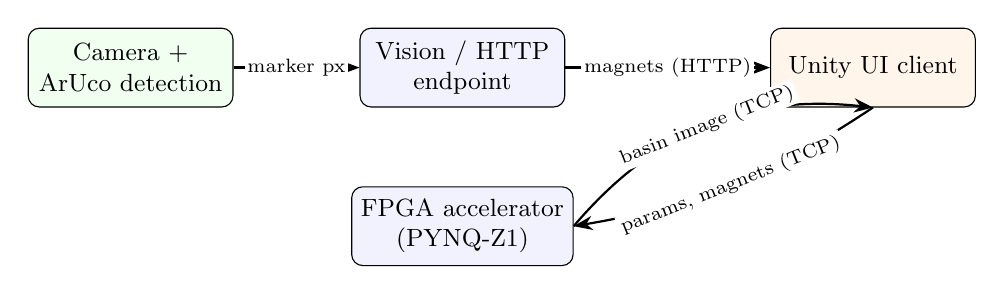
\begin{tikzpicture}[
  node distance=10mm and 16mm,
  box/.style={draw, rounded corners, align=center, minimum height=10mm,
              minimum width=26mm, font=\small, fill=blue!5},
  cam/.style={draw, rounded corners, align=center, minimum height=10mm,
              minimum width=26mm, font=\small, fill=green!6},
  ui/.style={draw, rounded corners, align=center, minimum height=10mm,
              minimum width=26mm, font=\small, fill=orange!8},
  arr/.style={-{Stealth[length=2.4mm]}, thick},
  lbl/.style={font=\scriptsize, fill=white, inner sep=1pt}
]
\node[cam] (cam) {Camera +\\ ArUco detection};
\node[box, right=of cam] (vision) {Vision / HTTP\\ endpoint};
\node[box, below=of vision] (fpga) {FPGA accelerator\\ (PYNQ-Z1)};
\node[ui, right=26mm of vision] (unity) {Unity UI client};

\draw[arr] (cam) -- node[lbl]{marker px} (vision);
\draw[arr] (vision) -- node[lbl, sloped]{magnets (HTTP)} (unity);
\draw[arr] (unity.south) to[bend left=12] node[lbl,sloped]{params, magnets (TCP)} (fpga.east);
\draw[arr] (fpga.east) to[bend left=28] node[lbl,sloped]{basin image (TCP)} (unity.south);
\end{tikzpicture}
\caption{System data flow. High-rate image and parameter traffic uses a binary
TCP protocol between Unity and the FPGA; magnet positions are produced by the
ArUco vision pipeline and consumed (then relayed) by Unity.}
\label{fig:dataflow}
\end{figure}

\subsection{Project Management}
\owned{whole team -- summarise framework, roles and contingencies here}
\todo{Add the role matrix, Gantt/Kanban summary and risk register. The
UI author's role: design and implementation of the Unity front end, the
binary TCP client, parameter-control UX, 2D/3D visualisation and the latency
instrumentation harness; collaboration on the wire protocol and coordinate
conventions shared with the FPGA and vision teams.}

% =========================================================================
\section{Mathematical Model and Reference}
\owned{maths/modelling team}
The Unity interface treats the FPGA output as opaque pixel data, but the
front-end design (colour palettes, height scaling, coordinate mapping and
parameter ranges) is driven by the model below, so it is summarised here for
self-containedness. \todo{Expand each subsection; the parameter values quoted
match the floating-point golden reference in the repository.}

\subsection{Continuous-Time Model}
The bob position $(x,y)$ obeys a damped oscillator with central restoring force
and an attractive force toward each in-plane magnet $i$ at $(a_i,b_i)$:
\begin{align}
\ddot{x} &= -\gamma\dot{x} - \omega^2 x
   - \sum_i \mu\,\frac{x-a_i}{\big((x-a_i)^2+(y-b_i)^2+h^2\big)^{3/2}}, \\
\ddot{y} &= -\gamma\dot{y} - \omega^2 y
   - \sum_i \mu\,\frac{y-b_i}{\big((x-a_i)^2+(y-b_i)^2+h^2\big)^{3/2}},
\end{align}
where $\gamma$ is the damping factor, $\omega^2$ the restoring coefficient,
$\mu$ the magnet strength and $h^2$ the squared bob--magnet plane separation
(kept positive to avoid a singularity). The golden reference uses
$\gamma=0.20$, $\omega^2=1.00$, $h^2=0.25$, $\mu=1.00$, and three magnets on an
equilateral triangle at $(1,0)$ and $(-\tfrac12,\pm\tfrac{\sqrt3}{2})$.

\subsection{Discrete-Time Approximation}
The reference integrates with semi-implicit (symplectic) Euler at step
$\Delta t = 0.01$:
\[
v_{n+1}=v_n+\Delta t\,a(x_n,v_n),\qquad x_{n+1}=x_n+\Delta t\,v_{n+1},
\]
which maps cleanly onto an FPGA datapath of registers, multipliers, adders and
a LUT/approximation for the inverse-power magnet term. \owned{FPGA team for the
hardware mapping}

\subsection{Settle and Timeout Conditions}
A pixel is classified once the bob stays within $r_\text{settle}=0.10$ of a
magnet \emph{and} below $v_\text{settle}=0.01$ in speed for
$3$ consecutive steps, or on timeout at $\text{max\_steps}=5000$. The iteration
count at settling is exported alongside the basin label and is what the Unity
3D view renders as height.

\subsection{Floating-Point Reference Model}
\owned{maths team} A NumPy float64 model is the functional golden reference;
\todo{cross-reference figure of the reference basin image.}

\subsection{Parameter Selection}
The render window is the square $[-1.8,1.8]^2$ in simulation units; this exact
constant ($1.8$) is reused throughout the Unity coordinate mappings and the
ArUco homography target so that pixel, simulation and board coordinates agree.
\todo{Justify word-length / bit-depth selection here (links to Section 4).}

% =========================================================================
\section{Accelerator Microarchitecture}
\owned{FPGA team -- full content}
\todo{This section is authored by the FPGA team. The only interface that the
Unity client depends on is summarised in Section~\ref{sec:protocol}: a binary
image frame (width, height, bit depth, version, packed pixels) and a parameter
register update. Keep the pixel encoding (Section~\ref{sec:pixeldecode}) in sync
with the hardware.}

\subsection{Pixel Scanner and Coordinate Mapper}\owned{FPGA team}
\subsection{Fixed-Point Number Representation}\owned{FPGA team}
\subsection{LUT-Based Force Approximation}\owned{FPGA team}
\subsection{Pipelined Pendulum Solver}\owned{FPGA team}
\subsection{Parallel Solver Architecture}\owned{FPGA team}
\subsection{AXI-Lite Control Interface}\owned{FPGA team}
\subsection{VDMA Data Transfer}\owned{FPGA team}

% =========================================================================
\section{Interactive Visualisation \& Control}

\subsection{Python/PYNQ Control Software}
\owned{PYNQ/vision team -- written here from the UI's perspective}
From the Unity client's perspective the control software provides two services.
First, a TCP server on the board accepts the binary protocol of
Section~\ref{sec:protocol}, forwards parameter and magnet updates to the
accelerator, and streams completed basin frames back. Second, the ArUco vision
pipeline (Section~\ref{sec:magnets}) detects physical magnet tokens, rectifies
their image coordinates onto the simulation plane via a homography, and exposes
them on a lightweight HTTP endpoint that Unity polls. \todo{PYNQ team to detail
the server, threading and overlay binding. The websocket hub
(\texttt{ws/\{client\}}) is the intended convergence point for ArUco, Unity and
FPGA clients and should be described if it is part of the final build.}

% -------------------------------------------------------------------------
\subsection{Unity-Based User Interface}
\label{sec:unity}

The user interface is a Unity application (Universal Render Pipeline) whose
responsibilities are: (i) maintain a robust connection to the FPGA;
(ii) present the basin image in two complementary visual forms; (iii) let the
user manipulate the model parameters with immediate visual feedback;
(iv) integrate physical magnet tracking; and (v) provide 2D/3D navigation.
The code is deliberately modular --- one ``concern'' per
\texttt{MonoBehaviour} --- so that the networking, control, rendering and
camera logic can be developed and tested independently. Table~\ref{tab:scripts}
lists the components.

\begin{table}[h]
\centering
\caption{Unity components and responsibilities.}
\label{tab:scripts}
\small
\begin{tabular}{@{}lp{10.4cm}@{}}
\toprule
\textbf{Script} & \textbf{Responsibility} \\
\midrule
\texttt{PynqConnection} & Background-threaded binary TCP client; frame
codec; auto-reconnect; outbound parameter/magnet sending; main-thread event
marshalling. \\
\texttt{PynqParamController} & Throttles and de-duplicates slider-driven
parameter updates before they are sent. \\
\texttt{SliderTextDisplay} & Maps a normalised UI slider to a physical
parameter range, formats the readout, raises change/release events. \\
\texttt{PendulumRenderer} & Decodes each pixel into (basin, iteration count);
builds the 2D category and value textures and the 3D height-field mesh. \\
\texttt{MagnetRenderer} & Polls the vision endpoint for magnet positions,
draws them on a mini-map, and relays them to the FPGA. \\
\texttt{PanZoom} & Pan/zoom of the 2D simulation window, constrained to the
valid simulation bounds. \\
\texttt{OrbitCamera} & Orbit/pan/zoom camera for the 3D surface view. \\
\texttt{ViewManager} & Switches between the 2D and 3D presentations. \\
\texttt{ImagePostToFrameTimer}, \texttt{SliderToImageTimer} & Latency
instrumentation (local render time and end-to-end round trip). \\
\texttt{VertexColor} (shader) & Minimal URP shader that renders the 3D mesh
using per-vertex basin colours. \\
\bottomrule
\end{tabular}
\end{table}

% --------------------------------------------------
\subsubsection{Networking layer and wire protocol}
\label{sec:protocol}

All latency-critical traffic uses a single persistent TCP connection
(\texttt{PynqConnection}). A custom binary framing was chosen over JSON-over-HTTP
because a basin frame is dense numeric data sent many times per second; framing
it as raw bytes avoids both per-frame connection overhead and the
serialisation cost of text formats. Every frame is:
\[
\underbrace{\texttt{type}}_{1\,\text{byte}}\;
\underbrace{\texttt{length}}_{4\,\text{bytes, big-endian}}\;
\underbrace{\texttt{payload}}_{\texttt{length bytes}}
\]
with message types \texttt{PARAMS} (\texttt{0x01}) and \texttt{MAGNETS}
(\texttt{0x02}) outbound, and \texttt{IMAGE} (\texttt{0x10}) and \texttt{INFO}
(\texttt{0x11}) inbound. An image payload begins with a 9-byte header
(\texttt{u16} width, \texttt{u16} height, \texttt{u8} bit depth, \texttt{u32}
version) followed by packed pixels (one byte each at $\le 8$ bits, otherwise
two bytes big-endian). Parameter and magnet payloads are compact JSON.

\paragraph{Threading.}
Networking runs on a dedicated background thread so that a blocking socket read
never stalls Unity's render loop. Decoded messages are pushed onto a
lock-free \texttt{ConcurrentQueue} and drained in \texttt{Update()}, guaranteeing
that all \texttt{ImageReceived}/\texttt{InfoReceived} events fire on the Unity
main thread where it is safe to touch \texttt{Texture2D} and \texttt{Mesh}
objects (Listing~\ref{lst:io}). The connection self-heals: on any socket error
the loop closes the stream, waits a configurable interval, and reconnects,
flushing any pending parameter frame on reconnection.

\begin{lstlisting}[language=Java,caption={Background receive loop drained on the main thread (\texttt{PynqConnection}).},label={lst:io}]
// background thread: read framed messages, enqueue for main thread
private void ReadFrames() {
    byte[] header = new byte[5];
    while (running) {
        ReadExactly(header, 5);
        byte type = header[0];
        int length = (int)ReadU32BE(header, 1);
        byte[] payload = length > 0 ? new byte[length] : Array.Empty<byte>();
        if (length > 0) ReadExactly(payload, length);
        if (type == MSG_IMAGE) inbound.Enqueue(DecodeImage(payload));
        else if (type == MSG_INFO) inbound.Enqueue(DecodeInfo(payload));
    }
}
// main thread (Update): raise events where Unity objects are safe to touch
while (inbound.TryDequeue(out object msg)) { /* invoke ImageReceived / InfoReceived */ }
\end{lstlisting}

\paragraph{Frame versioning.}
Each parameter update carries an incrementing \texttt{version}, and the client
records the minimum image version it is willing to accept afterwards. Incoming
frames older than this watermark are discarded in \texttt{PendulumRenderer}, so
the display never briefly shows a stale basin produced before the latest slider
change took effect --- important when the user drags a slider and several
in-flight frames are still arriving.

% --------------------------------------------------
\subsubsection{Parameter control and UX}
\label{sec:params}

Four parameters --- damping factor, magnet strength, pendulum length and
pendulum height --- are exposed as sliders. \texttt{SliderTextDisplay} maps the
slider's normalised $[0,1]$ value onto the parameter's physical
$[\text{min},\text{max}]$ range, rounds to two decimals for a stable readout,
and raises two signals: a \emph{changed} signal on every move and a
\emph{released} signal on pointer-up.

A na\"ive design would transmit a parameter frame on every slider callback,
flooding the link and the accelerator while the user drags. Instead,
\texttt{PynqParamController} \textbf{throttles} sends to at most one every
\SI{0.1}{s} while dragging, and on release forces an immediate final send so the
last value is never lost. It also \textbf{de-duplicates}: if a snapshot equals
the last value actually sent (or a value already queued), it is dropped. This
gives responsive dragging without saturating the FPGA, and guarantees the steady
state always reflects the slider exactly. The combination of throttle +
forced-flush-on-release is a deliberate latency/throughput trade-off and is
discussed in Section~\ref{sec:tradeoffs}.

% --------------------------------------------------
\subsubsection{Basin visualisation: 2D textures and 3D surface}
\label{sec:pixeldecode}

\texttt{PendulumRenderer} subscribes to \texttt{ImageReceived} and, for each
frame, converts the packed pixels into three views. Every pixel encodes two
quantities: the \emph{basin label} (which magnet won) and the \emph{iteration
count} (how long the bob took to settle, i.e.\ how close to a boundary the
starting point was). The decode is bit-depth aware so the same front end works
with the current 6-bit hardware output and a future 14-bit mode:

\begin{lstlisting}[language=Java,caption={Bit-depth-aware pixel decode (\texttt{PendulumRenderer}).},label={lst:decode}]
static void DecodePixel(int pixel, int bitDepth, out int category, out int depth) {
    if (bitDepth <= 6) { category = pixel & 0x3;          depth = (pixel >> 2) & 0xF; }
    else               { category = (pixel >> 12) & 0x3;  depth = pixel & 0xFFF; }
}
\end{lstlisting}

\paragraph{2D category map.}
The basin label indexes a small palette (one colour per magnet, dark grey for
unresolved), producing the familiar tri-colour basin image. Array rows are
flipped vertically to match Unity's bottom-left texture origin.

\paragraph{2D value map.}
The iteration count is normalised to $[0,255]$ and passed through a
\emph{plasma} colour map (a perceptually-ordered gradient interpolated between
nine anchor colours). This exposes the fractal boundary structure --- regions
that take many iterations to settle glow brightly --- which the flat category
map hides.

\paragraph{3D height field.}
The same per-pixel data builds a triangulated mesh: $(x,y)$ are the pixel
coordinates and the height is the iteration count, scaled per bit depth. Vertices
are coloured by basin label and drawn with the minimal \texttt{VertexColor} URP
shader, giving an interactive 3D ``landscape'' whose peaks are the
sensitive basin boundaries. A \texttt{UInt32} index buffer is used so the mesh
can exceed 65k vertices at full resolution, and the mesh skeleton (triangle
indices) is rebuilt only when the frame dimensions change, not every frame.

% --------------------------------------------------
\subsubsection{Physical magnet tracking integration}
\label{sec:magnets}

\texttt{MagnetRenderer} closes the loop between the physical board and the
simulation. It polls the vision endpoint (default every \SI{0.5}{s}) for the
current magnet dictionary, maps each magnet's simulation coordinate
($[-1.8,1.8]$) onto a $130\times130$ mini-map and draws it as a coloured disc,
then relays the same coordinates to the FPGA over TCP
(\texttt{SendMagnets}). The vision side derives these coordinates from ArUco
markers: four corner markers (IDs 0--3) define a homography that rectifies the
camera image to the square board, and three token markers (IDs 4--6) are the
movable magnets, whose centres are transformed into simulation units before
publishing. Because Unity both \emph{displays} and \emph{forwards} the magnet
positions, the on-screen dots and the FPGA's computed basin are always
consistent.

% --------------------------------------------------
\subsubsection{Navigation and view management}

Two camera/navigation behaviours serve the two views. \texttt{PanZoom} (2D)
implements scroll-to-zoom and drag-to-pan over the simulation window using
Unity's Input System, clamping the requested window so it can never leave the
valid simulation bounds $[-1.8,1.8]^2$ (a minimum half-size prevents zooming in
past the point where the image becomes blocky). \texttt{OrbitCamera} (3D)
provides orbit (left-drag), pan (right-drag) and zoom (scroll) around the height
field. \texttt{ViewManager} toggles between the 2D canvas and the 3D overlay,
enabling the orbit camera only in 3D. \todo{Confirm whether the pan/zoom window
is forwarded to the FPGA to re-render at higher resolution, or is a local
view-only crop; describe accordingly.}

% --------------------------------------------------
\subsubsection{Design decisions and trade-offs}
\label{sec:tradeoffs}

\begin{itemize}[noitemsep]
  \item \textbf{Binary TCP vs.\ HTTP/JSON for frames.} Dense, high-rate pixel
        data is sent as packed bytes over one persistent socket, eliminating
        per-frame connection setup and text-parsing overhead. Low-rate,
        human-readable data (parameters, magnets) stays as small JSON payloads
        inside the same framing for convenience.
  \item \textbf{Background I/O + main-thread marshalling.} Keeps the render loop
        free of blocking socket calls while respecting Unity's rule that scene
        objects are touched only on the main thread.
  \item \textbf{Throttle + de-duplicate + flush-on-release.} Bounds the
        parameter update rate during dragging (protecting the link and the
        accelerator) while guaranteeing the final value always lands.
  \item \textbf{Frame versioning watermark.} Prevents stale frames from
        flashing on screen after a parameter change, at the cost of occasionally
        discarding a just-too-old frame.
  \item \textbf{Bit-depth-aware decode.} One renderer supports both the present
        6-bit and a future 14-bit hardware output without code changes,
        decoupling UI development from the FPGA's numeric format.
  \item \textbf{Two visual encodings + 3D.} The category map answers ``which
        magnet?'', the plasma value map and 3D surface answer ``how chaotic
        here?'', directly serving the educational objective.
\end{itemize}

% =========================================================================
\section{Verification and Evaluation}

\subsection{Evaluation Strategy Linked to Design Objectives}
The UI's objectives --- responsiveness, faithful presentation of the
accelerator output, robust connectivity and intuitive control --- map onto
measurable tests: end-to-end latency (slider-to-image), local render time,
reconnection behaviour, and correctness of the pixel decode against the golden
reference. \todo{Tabulate each requirement against its test and pass criterion.}

\subsection{Software Model Validation}
\owned{maths team} Validation of the floating-point reference and the
fixed-point model against it. \todo{cross-reference.}

\subsection{Submodule Testing}
The Python services that the UI depends on are unit-tested (the Flask state
model, magnet add/remove/update, parameters and \texttt{/info} construction have
a \texttt{pytest} suite). On the Unity side, the pixel decode and coordinate
mappings are deterministic pure functions and were checked against the golden
reference's encoding; the networking codec was exercised against
\todo{describe: loopback test / recorded frames}. \todo{Add ArUco accuracy test
(reprojection error of known marker layout).}

\subsection{System Performance Evaluation}
Two lightweight stopwatches instrument the live system without external tools.
\texttt{SliderToImageTimer} starts when a slider changes and stops when an image
with a newer version is rendered, giving the \textbf{end-to-end round-trip
latency} (UI $\rightarrow$ FPGA $\rightarrow$ UI). \texttt{ImagePostToFrameTimer}
measures the \textbf{local processing time} from a TCP frame arriving to the
textures and mesh being updated, isolating the UI's own contribution from the
network/compute path. Together they decompose total latency into ``UI render''
and ``everything else''. \todo{Insert the measured distributions (median,
p95) for 6-bit $160\times120$ frames; compare 2D-only vs.\ 2D+3D rendering
cost; state the achieved interactive frame rate.}

% =========================================================================
\section*{References}
\todo{Add bibliography (PYNQ docs, ArUco/OpenCV, Unity URP, plasma colormap
source). Consider switching to \texttt{biblatex} when integrating with the team
document.}

% =========================================================================
\appendix
\section{Wire Protocol Summary}
\begin{table}[h]
\centering
\small
\begin{tabular}{@{}llp{7.6cm}@{}}
\toprule
\textbf{Type} & \textbf{Dir} & \textbf{Payload} \\
\midrule
\texttt{0x01 PARAMS}  & UI$\to$FPGA & JSON: version, dampingFactor,
magneticStrength, pendulumLength, pendulumHeight \\
\texttt{0x02 MAGNETS} & UI$\to$FPGA & JSON: \{ magnets: \{ magnet\_i: \{x,y\} \} \} \\
\texttt{0x10 IMAGE}   & FPGA$\to$UI & 9-byte header (w,h,depth,version) +
packed pixels \\
\texttt{0x11 INFO}    & FPGA$\to$UI & JSON: magnet dictionary \\
\bottomrule
\end{tabular}
\caption{Binary framing: 1-byte type, 4-byte big-endian length, payload.}
\end{table}

\section{Key Source Files}
\todo{Optionally include trimmed listings of \texttt{PynqConnection.cs},
\texttt{PendulumRenderer.cs} and \texttt{PynqParamController.cs}, or reference
the repository.}

\end{document}
